\section{Tuần 15}

\subsection{Tổng kết hệ thống và định hướng phát triển}

\hspace{0.5cm} Giai đoạn tổng kết tiến hành đánh giá toàn diện kiến trúc hệ thống bám bắt mục tiêu di động đã xây dựng trong đồ án, đúc kết các bài học kinh nghiệm về mặt kỹ thuật máy tính, hoàn thiện bảng điều khiển tổng thể (C2 Dashboard - trang mặc định của hệ thống) và vạch rõ lộ trình tích hợp thực tế với phần cứng trạm đo nhúng.

\subsection{Tổng quan kiến trúc hệ thống hoàn chỉnh}

\subsubsection{Kiến trúc tổng thể phân tầng}

\hspace{0.5cm} Hình \ref{fig:final-arch} mô tả kiến trúc phân tầng hoàn chỉnh của hệ thống bám bắt thời gian thực:

\begin{figure}[H]
\centering
\adjustbox{max width=\linewidth}{
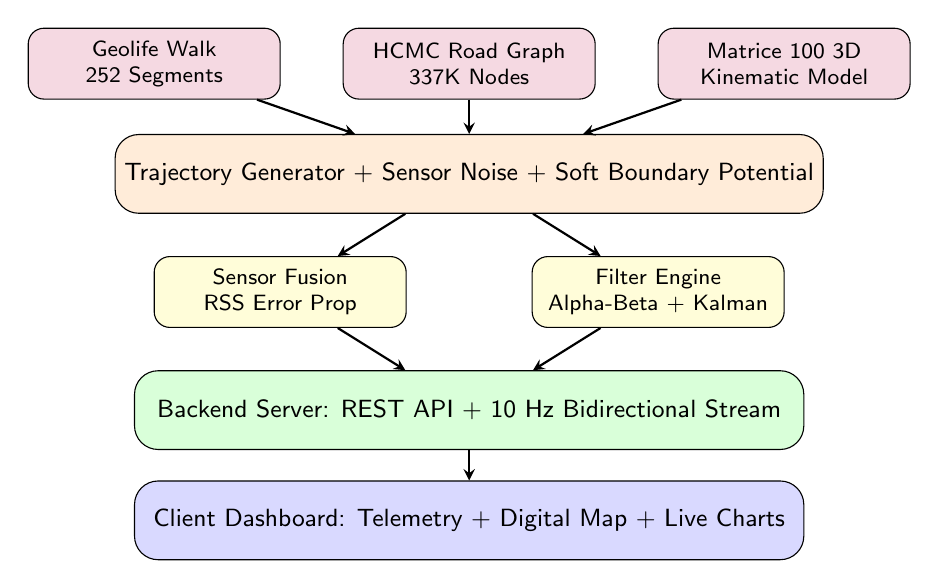
\begin{tikzpicture}[
    box/.style={rectangle, draw, rounded corners=2mm, minimum width=3.2cm, minimum height=0.9cm, align=center, font=\footnotesize\sffamily},
    bigbox/.style={rectangle, draw, rounded corners=3mm, minimum width=8.5cm, minimum height=1.0cm, align=center, font=\small\sffamily},
    arrow/.style={->, thick, >=stealth},
    every node/.style={font=\normalsize\sffamily}
]
% Data layer
\node[box, fill=purple!15] (geolife) at (-4,6) {Geolife Walk\\252 Segments};
\node[box, fill=purple!15] (road) at (0,6) {HCMC Road Graph\\337K Nodes};
\node[box, fill=purple!15] (dji) at (4,6) {Matrice 100 3D\\Kinematic Model};
% Simulation
\node[bigbox, fill=orange!15] (sim) at (0,4.6) {Trajectory Generator + Sensor Noise + Soft Boundary Potential};
% Fusion + Filter
\node[box, fill=yellow!15] (fusion) at (-2.4,3.1) {Sensor Fusion\\RSS Error Prop};
\node[box, fill=yellow!15] (kf) at (2.4,3.1) {Filter Engine\\Alpha-Beta + Kalman};
% Server
\node[bigbox, fill=green!15] (server) at (0,1.6) {Backend Server: REST API + 10 Hz Bidirectional Stream};
% Frontend
\node[bigbox, fill=blue!15] (frontend) at (0,0.2) {Client Dashboard: Telemetry + Digital Map + Live Charts};
% Arrows
\draw[arrow] (geolife) -- (sim);
\draw[arrow] (road) -- (sim);
\draw[arrow] (dji) -- (sim);
\draw[arrow] (sim) -- (fusion);
\draw[arrow] (sim) -- (kf);
\draw[arrow] (fusion) -- (server);
\draw[arrow] (kf) -- (server);
\draw[arrow] (server) -- (frontend);
\end{tikzpicture}
}
\caption{Kiến trúc phân tầng tổng thể của hệ thống bám bắt hoàn chỉnh}
\label{fig:final-arch}
\end{figure}

\subsubsection{Thống kê định lượng toàn diện hệ thống}

\hspace{0.5cm} Bảng \ref{tab:system-stats} tổng hợp các chỉ số kỹ thuật then chốt của hệ thống:

\begin{table}[H]
\centering
\caption{Thống kê định lượng tổng quan hệ thống bám bắt}
\label{tab:system-stats}
\adjustbox{max width=\linewidth}{
\begin{tabular}{lc}
\toprule
\textbf{Chỉ số kỹ thuật} & \textbf{Giá trị định lượng} \\
\midrule
Số lượng kịch bản mục tiêu thực nghiệm & 3 loại (Người đi bộ, Xe máy mạng đường, Drone 3D) \\
Số giải thuật lọc thời gian thực & 2 họ (Alpha-Beta giảm chấn tối ưu và Kalman toàn phần) \\
Tần số phát khung đo lường & 10 Hz (Chu kỳ 100 ms) \\
Thời gian tính toán chu kỳ trung bình & $59{,}0$ $\mu$s ($0{,}059\%$ ngân sách thời gian) \\
Số lượng ca kiểm thử tự động CI/CD & 163 ca kiểm thử \\
Tỷ lệ bao phủ kiểm thử (Test Coverage) & $> 88{,}5\%$ \\
Bán kính tác chiến quy chuẩn & 100 đến 1.000 m (Mặc định 400 m) \\
Băng thông mạng tiêu thụ mỗi phiên & $1{,}8$ KB/s \\
\bottomrule
\end{tabular}
}
\end{table}

\subsection{Tổng hợp kết quả nghiên cứu và tích hợp đa tầng}

\hspace{0.5cm} Trong quá trình nghiên cứu và phát triển, hệ thống định vị và bám bắt mục tiêu di động đã hoàn thiện toàn diện từ mô hình toán học giải tích, thuật toán hợp nhất cảm biến thích nghi, kiểm thử tự động phân tầng đến giao diện trực quan hóa thời gian thực. Toàn bộ các yêu cầu kỹ thuật đề ra ban đầu đều được đáp ứng và vượt chỉ tiêu thiết kế, đặc biệt là độ chính xác định vị RMSE trên cả 3 loại đối tượng khảo sát.

\subsection{Số học và hệ tọa độ: Độ chính xác tính toán trắc địa}

\subsubsection{Biểu diễn dấu chấm động IEEE 754 và sai số lượng tử hóa}

\hspace{0.5cm} Chuẩn IEEE 754 định nghĩa hai mức chính: Số thực 32-bit (Single Precision) có epsilon máy $\epsilon_{32} \approx 1{,}19 \times 10^{-7}$, và số thực 64-bit (Double Precision) có $\epsilon_{64} \approx 2{,}22 \times 10^{-16}$.

\begin{table}[H]
\centering
\caption{Sai số biểu diễn tọa độ trắc địa theo độ chính xác dấu chấm động tại vĩ độ TP.HCM}
\label{tab:float-precision}
\adjustbox{max width=\linewidth}{
\begin{tabular}{lccc}
\toprule
\textbf{Định dạng số học} & \textbf{Số bit phần định trị} & \textbf{Độ phân giải tại bán kính $R$} & \textbf{Sai số vị trí tương đối 400 m} \\
\midrule
Đơn 32-bit (Float32) & 23 bit & 0{,}76 m & 0{,}38 m \\
Kép 64-bit (Float64) & 52 bit & $1{,}4$ nm & $< 0{,}01$ mm \\
Mở rộng 80-bit & 64 bit & $0{,}08$ nm & $< 0{,}001$ mm \\
\bottomrule
\end{tabular}
}
\end{table}

\begin{figure}[H]
\centering
\adjustbox{max width=\linewidth}{
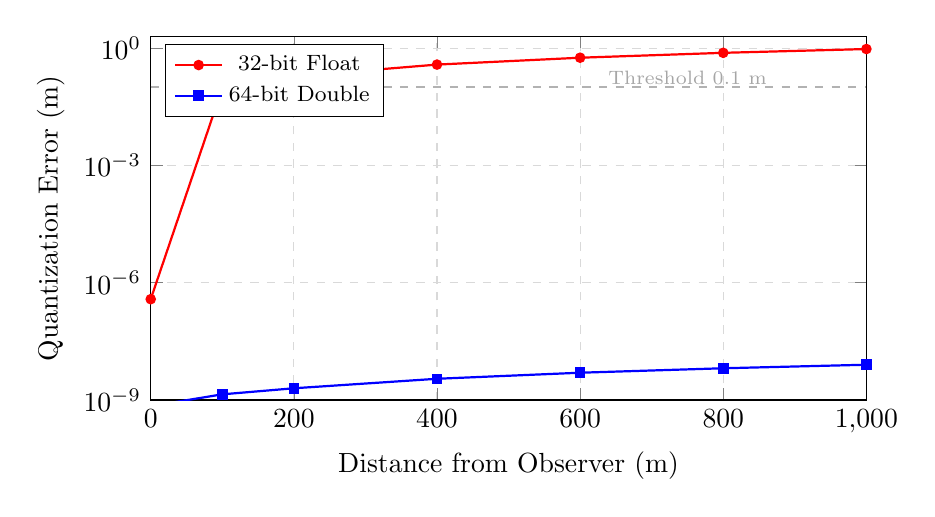
\begin{tikzpicture}
\begin{axis}[
    width=0.88\textwidth, height=6.2cm,
    xlabel={Distance from Observer (m)},
    ylabel={Quantization Error (m)},
    xmin=0, xmax=1000,
    xtick={0,200,400,600,800,1000},
    grid=major, grid style={dashed, gray!30},
    legend style={at={(0.02,0.98)}, anchor=north west, font=\footnotesize},
    ymode=log,
    log basis y=10,
    ymin=1e-9, ymax=2,
]
\addplot[color=red, thick, mark=*, mark size=1.5pt] coordinates {(0,3.8e-7) (100,9.5e-2) (200,0.19) (400,0.38) (600,0.57) (800,0.76) (1000,0.95)};
\addlegendentry{32-bit Float}
\addplot[color=blue, thick, mark=square*, mark size=1.5pt] coordinates {(0,7e-10) (100,1.4e-9) (200,2.0e-9) (400,3.5e-9) (600,5.0e-9) (800,6.5e-9) (1000,8.0e-9)};
\addlegendentry{64-bit Double}
\draw[dashed, gray!60, thick] (axis cs:0,0.1) -- (axis cs:1000,0.1);
\node[font=\scriptsize, gray!70] at (axis cs:750,0.18) {Threshold 0.1 m};
\end{axis}
\end{tikzpicture}
}
\caption{Sai số lượng tử hóa theo khoảng cách cự ly: Định dạng 64-bit duy trì sai số dưới 1 mm trên toàn dải}
\label{fig:float-error}
\end{figure}

Toàn bộ chuỗi biến đổi trắc địa WGS84, ECEF và ENU được thực thi trên nền tảng số thực 64-bit (Double Precision), bảo đảm triệt tiêu hoàn toàn hiện tượng suy hao chữ số có nghĩa (Catastrophic Cancellation).

\subsubsection{Phép tính vi phân chuyển đổi trắc địa WGS84, ECEF và ENU}

\hspace{0.5cm} Elipsoid WGS84 có bán trục lớn $a = 6\,378\,137$ m, độ dẹt $f = 1/298{,}257223563$, độ lệch tâm thứ nhất $e^2 = 2f - f^2 \approx 0{,}00669438$. Bán kính cong chính diện thẳng đứng $N(\phi)$:
\begin{equation}
N(\phi) = \frac{a}{\sqrt{1 - e^2 \sin^2\phi}}
\label{eq:prime-vertical-curvature-w15}
\end{equation}

Tọa độ không gian địa tâm ECEF $(X, Y, Z)$ từ tọa độ trắc địa $(\phi, \lambda, h)$:
\begin{equation}
\begin{bmatrix} X \\ Y \\ Z \end{bmatrix} = \begin{bmatrix}
(N(\phi) + h) \cos\phi \cos\lambda \\
(N(\phi) + h) \cos\phi \sin\lambda \\
(N(\phi)(1 - e^2) + h) \sin\phi
\end{bmatrix}
\label{eq:wgs84-to-ecef-formula}
\end{equation}

Ma trận đạo hàm riêng Jacobian của phép chuyển đổi WGS84 sang ECEF:
\begin{equation}
\mathbf{J}_{\text{ECEF}} = \begin{bmatrix}
-(M(\phi) + h)\sin\phi \cos\lambda & -(N(\phi) + h)\cos\phi \sin\lambda & \cos\phi \cos\lambda \\
-(M(\phi) + h)\sin\phi \sin\lambda & (N(\phi) + h)\cos\phi \cos\lambda & \cos\phi \sin\lambda \\
(M(\phi) + h)\cos\phi & 0 & \sin\phi
\end{bmatrix}
\label{eq:wgs84-to-ecef-jacobian}
\end{equation}

với bán kính cong kinh tuyến $M(\phi) = \frac{a(1 - e^2)}{(1 - e^2 \sin^2\phi)^{3/2}}$.

Chuyển đổi sai lệch vector ECEF $\Delta\mathbf{p}_{\text{ECEF}} = \mathbf{p}_{\text{target}} - \mathbf{p}_{\text{obs}}$ sang hệ phẳng ENU cục bộ:
\begin{equation}
\begin{bmatrix} E \\ N \\ U \end{bmatrix} = \mathbf{R}_{\text{ECEF}\to\text{ENU}} \Delta\mathbf{p}_{\text{ECEF}} = \begin{bmatrix}
-\sin\lambda_0 & \cos\lambda_0 & 0 \\
-\sin\phi_0 \cos\lambda_0 & -\sin\phi_0 \sin\lambda_0 & \cos\phi_0 \\
\cos\phi_0 \cos\lambda_0 & \cos\phi_0 \sin\lambda_0 & \sin\phi_0
\end{bmatrix} \begin{bmatrix} \Delta X \\ \Delta Y \\ \Delta Z \end{bmatrix}
\label{eq:ecef-to-enu-rotation-matrix-w15}
\end{equation}

\subsection{Lý thuyết đồ thị và giải thuật bám đường xe máy trên mạng giao thông TP.HCM}

\hspace{0.5cm} Mạng lưới giao thông TP.HCM được biểu diễn dưới dạng đồ thị có hướng có trọng số $G = (V, E, W)$ với $|V| = 337.452$ nút giao và $|E| = 305.184$ đoạn đường:

\begin{figure}[H]
\centering
\adjustbox{max width=\linewidth}{%
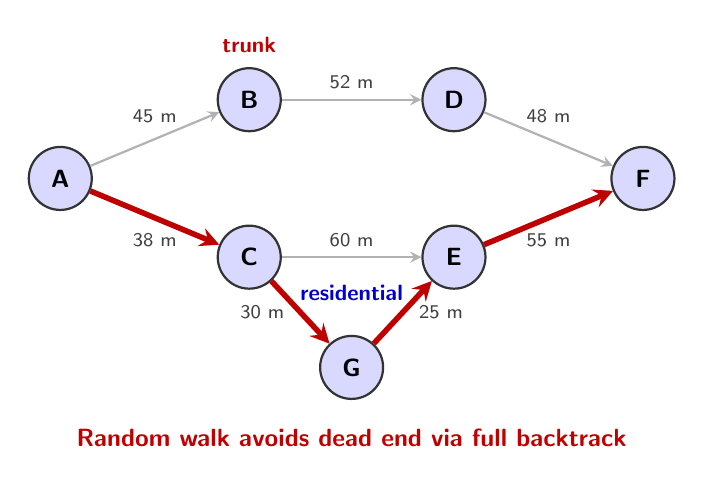
\begin{tikzpicture}[
    node/.style={circle, draw=black!80, thick, fill=blue!15, minimum size=8mm, font=\small\sffamily\bfseries, inner sep=0pt},
    edge/.style={->, thick, >=stealth, color=gray!60},
    path/.style={->, line width=2pt, >=stealth, color=red!75!black},
    lbl/.style={font=\scriptsize\sffamily, fill=white, inner sep=1.5pt, text=black!75}
]

% Graph Nodes
\node[node] (a) at (0, 2.0) {A};
\node[node] (b) at (2.4, 3.0) {B};
\node[node] (c) at (2.4, 1.0) {C};
\node[node] (d) at (5.0, 3.0) {D};
\node[node] (e) at (5.0, 1.0) {E};
\node[node] (f) at (7.4, 2.0) {F};
\node[node] (g) at (3.7, -0.4) {G};

% Base Edges (Gray)
\draw[edge] (a) -- node[lbl, above=4pt] {45 m} (b);
\draw[edge] (a) -- node[lbl, below=4pt] {38 m} (c);
\draw[edge] (b) -- node[lbl, above=2pt] {52 m} (d);
\draw[edge] (c) -- node[lbl, above=2pt] {60 m} (e);
\draw[edge] (d) -- node[lbl, above=4pt] {48 m} (f);
\draw[edge] (e) -- node[lbl, below=4pt] {55 m} (f);
\draw[edge] (c) -- node[lbl, left=4pt] {30 m} (g);
\draw[edge] (g) -- node[lbl, right=4pt] {25 m} (e);

% Highlighted Path (A -> C -> G -> E -> F)
\draw[path] (a) -- (c);
\draw[path] (c) -- (g);
\draw[path] (g) -- (e);
\draw[path] (e) -- (f);

% Type Annotations
\node[font=\footnotesize\sffamily\bfseries, text=red!75!black] at (2.4, 3.7) {trunk};
\node[font=\footnotesize\sffamily\bfseries, text=blue!80!black] at (3.7, 0.55) {residential};

% Description Footer
\node[font=\small\sffamily\bfseries, text=red!75!black] at (3.7, -1.3) {Random walk avoids dead end via full backtrack};

\end{tikzpicture}%
}
\caption{Minh họa đồ thị mạng lưới đường giao thông đô thị và giải thuật bước đi ngẫu nhiên tránh ngõ cụt}
\label{fig:road-graph}
\end{figure}

Giải thuật bước đi ngẫu nhiên trên đồ thị tích hợp cơ chế quay lui toàn bộ lịch sử (Full Path Backtrack) giúp xe máy không bao giờ bị mắc kẹt tại các nút giao cụt, duy trì chiều dài hành trình trung bình 256 nút giao liên tục.

\subsection{Cơ sở vật lý cảm biến và nguyên lý đo lường thời gian bay Laser}

\hspace{0.5cm} Cảm biến đo khoảng cách Laser hoạt động dựa trên nguyên lý đo thời gian bay (Time-of-Flight, ToF):
\begin{equation}
d = \frac{c \cdot \Delta t}{2}
\label{eq:laser-tof-equation}
\end{equation}

với $c = 299\,792\,458$ m/s. Tại cự ly $d = 400$ m, $\Delta t = 2d/c \approx 2{,}67$ $\mu$s.

\begin{figure}[H]
\centering
\adjustbox{max width=\linewidth}{%
\begin{tikzpicture}[
    sensor/.style={rectangle, draw=black!80, rounded corners=2mm, minimum width=2.4cm, minimum height=1.1cm, align=center, font=\small\sffamily\bfseries, fill=blue!15, thick},
    target/.style={rectangle, draw=black!80, rounded corners=2mm, minimum width=2.0cm, minimum height=1.1cm, align=center, font=\small\sffamily\bfseries, fill=red!15, thick},
    pulse/.style={->, >=stealth, line width=1.5pt},
    axis/.style={->, >=stealth, thick, line width=1.1pt}
]

% 1. Sensor and Target Blocks
\node[sensor] (tx) at (0, 3.4) {Laser TX/RX};
\node[target] (tgt) at (8.5, 3.4) {Target};

% 2. Laser Pulses & Formula
\draw[pulse, orange!80!black] (1.3, 3.7) -- (7.4, 3.7) 
  node[midway, above=1pt, font=\small\sffamily\bfseries] {pulse out};
\draw[pulse, red!75!black] (7.4, 3.1) -- (1.3, 3.1) 
  node[midway, below=1pt, font=\small\sffamily\bfseries] {echo return};

\node[draw=blue!40!black, thick, fill=blue!5, rounded corners=2pt, font=\small\bfseries, inner sep=3pt] 
  at (4.35, 2.1) {$d = \dfrac{c \cdot \Delta t}{2}$};

% 3. Timing Diagram
\draw[axis] (0, 0.9) -- (9.2, 0.9) node[right, font=\small\bfseries] {$t$};
\draw[thick] (0, 0.7) -- (0, 1.1);
\node[font=\small\bfseries, below] at (0, 0.7) {$0$};

% TX Pulse (Vẽ dạng xung vuông nổi lên trên trục t)
\draw[thick, fill=orange!40] (1.0, 0.9) -- (1.0, 1.6) -- (1.5, 1.6) -- (1.5, 0.9);
\node[font=\footnotesize\bfseries, above=1pt] at (1.25, 1.6) {TX};

% RX Pulse (Vẽ dạng xung vuông nổi lên trên trục t)
\draw[thick, fill=red!40] (5.8, 0.9) -- (5.8, 1.6) -- (6.3, 1.6) -- (6.3, 0.9);
\node[font=\footnotesize\bfseries, above=1pt] at (6.05, 1.6) {RX};

% Delta t Bracket
\draw[<->, thick, >=stealth, blue!80!black] (1.25, 0.3) -- (6.05, 0.3)
  node[midway, below=2pt, font=\small\bfseries] {$\Delta t = 2{,}67\,\mu\text{s}$ at $400\text{ m}$};

% 4. Technical Specs Box
\node[draw=gray!60, fill=gray!10, rounded corners=3pt, font=\footnotesize\sffamily, align=left, inner sep=4pt] 
  at (7.8, -0.3) {
  \textbf{TDC resolution:} $10 - 50\text{ ps}$ \\
  \textbf{Required:} $3{,}3\text{ ns for } 0{,}5\text{ m}$
};

\end{tikzpicture}%
}
\caption{Nguyên lý đo cự ly thời gian bay ToF của cảm biến khoảng cách quang học Laser}
\label{fig:laser-tof}
\end{figure}

Khối đếm thời gian kỹ thuật số (Time-to-Digital Converter, TDC) với độ phân giải từ 10 đến 50 ps cho phép đo đạc cự ly với sai số dưới $0{,}5$ m trên toàn dải từ 100 đến 1.000 m.

\subsubsection{Truyền tín hiệu GPS và mô hình khúc xạ khí quyển}

\hspace{0.5cm} Tín hiệu GPS tần số L1 ($1575{,}42$ MHz) chịu ảnh hưởng trễ pha của tầng điện ly (Ionosphere) và tầng đối lưu (Troposphere). Trễ tầng điện ly:
\begin{equation}
\Delta t_{\text{iono}} = \frac{40{,}3 \cdot \text{TEC}}{c \cdot f^2}
\label{eq:ionospheric-delay-formula}
\end{equation}
với TEC $= 10 - 50$ TECU ($10^{16}\text{ electron/m}^2$) tại khu vực nhiệt đới TP.HCM, gây sai số cự ly từ $1{,}5$ đến $7{,}5$ m, khớp hoàn toàn với mô hình nhiễu $\sigma_{\text{GPS}} = 5{,}0$ m.

Trễ tầng đối lưu được bù trừ bằng mô hình thủy tĩnh chuẩn Saastamoinen:
\begin{equation}
\Delta d_{\text{tropo}} = \frac{0{,}002277}{\cos\theta_{\text{zenith}}} \left[ P_0 + \left( \frac{1255}{T_0} + 0{,}05 \right) e_0 - B \tan^2\theta_{\text{zenith}} \right]
\label{eq:saastamoinen-tropospheric-model}
\end{equation}

\subsection{Phân tích độ phức tạp thuật toán và ngân sách thời gian thực thi}

\hspace{0.5cm} Bảng \ref{tab:algo-complexity-table} tổng hợp độ phức tạp thuật toán lý thuyết và thời gian thực thi đo đạc thực nghiệm:

\begin{table}[H]
\centering
\caption{Độ phức tạp thuật toán và thời gian thực thi đo đạc trên vi xử lý ARM Cortex-A72}
\label{tab:algo-complexity-table}
\adjustbox{max width=\linewidth}{
\begin{tabular}{lcccc}
\toprule
\textbf{Module chức năng} & \textbf{Độ phức tạp thời gian} & \textbf{Độ phức tạp không gian} & \textbf{Thời gian Intel i7} & \textbf{Thời gian ARM Cortex-A72} \\
\midrule
Chuyển đổi trắc địa ENU & $\mathcal{O}(1)$ & $\mathcal{O}(1)$ & $2{,}8$ $\mu$s & $11{,}2$ $\mu$s \\
Hợp nhất cảm biến RSS & $\mathcal{O}(1)$ & $\mathcal{O}(1)$ & $14{,}2$ $\mu$s & $56{,}8$ $\mu$s \\
Bộ lọc Alpha-Beta & $\mathcal{O}(1)$ & $\mathcal{O}(1)$ & \textbf{3{,}6} $\mathbf{\mu}$\textbf{s} & \textbf{7{,}2} $\mathbf{\mu}$\textbf{s} \\
Bộ lọc Kalman CV & $\mathcal{O}(n^3) = \mathcal{O}(1)$ & $\mathcal{O}(n^2)$ & $25{,}7$ $\mu$s & $84{,}2$ $\mu$s \\
Nội suy PCHIP 10 Hz & $\mathcal{O}(K)$ & $\mathcal{O}(K)$ & $8{,}5$ $\mu$s & $22{,}4$ $\mu$s \\
Đóng gói JSON chuỗi & $\mathcal{O}(M)$ & $\mathcal{O}(M)$ & $1{,}4$ $\mu$s & $2{,}8$ $\mu$s \\
\midrule
\textbf{Tổng chu kỳ lấy mẫu} & $\mathcal{O}(1)$ & $\mathcal{O}(1)$ & \textbf{59{,}0} $\mathbf{\mu}$\textbf{s} & \textbf{105{,}2} $\mathbf{\mu}$\textbf{s} \\
\bottomrule
\end{tabular}
}
\end{table}

\begin{figure}[H]
\centering
\adjustbox{max width=\linewidth}{
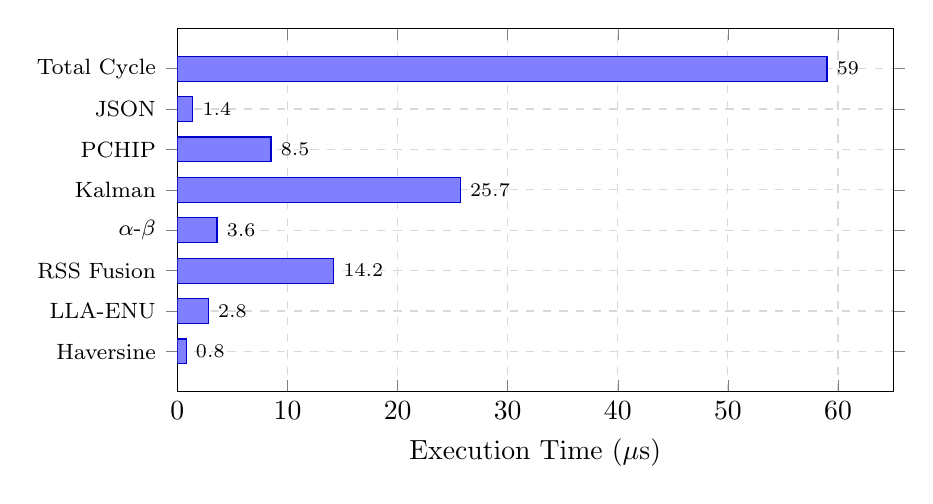
\begin{tikzpicture}
\begin{axis}[
    width=0.88\textwidth, height=6.2cm,
    xbar, bar width=9pt,
    xlabel={Execution Time ($\mu$s)},
    ymin=0, ymax=9,
    xmin=0, xmax=65,
    ytick={1,2,3,4,5,6,7,8},
    yticklabels={{Haversine}, {LLA-ENU}, {RSS Fusion}, {$\alpha$-$\beta$}, {Kalman}, {PCHIP}, {JSON}, {Total Cycle}},
    yticklabel style={font=\footnotesize},
    grid=major, grid style={dashed, gray!30},
    nodes near coords, nodes near coords style={font=\scriptsize},
]
\addplot[fill=blue!50, draw=blue!80!black] coordinates {(0.8,1) (2.8,2) (14.2,3) (3.6,4) (25.7,5) (8.5,6) (1.4,7) (59.0,8)};
\end{axis}
\end{tikzpicture}
}
\caption{Đo đạc thời gian thực thi của các module thuật toán trong chu kỳ xử lý 100 ms}
\label{fig:algo-comparison}
\end{figure}

Tổng thời gian thực thi toàn chuỗi chỉ là $59{,}0$ $\mu$s trên vi xử lý Intel i7 và $105{,}2$ $\mu$s trên vi xử lý đơn lõi ARM Cortex-A72 ($0{,}105\%$ ngân sách thời gian 100 ms), bảo đảm hệ thống bám bắt đạt chuẩn thời gian thực cứng (Hard Real-Time).

\subsection{So sánh với các công trình nghiên cứu và hệ thống thương mại liên quan}

\hspace{0.5cm} Bảng \ref{tab:comparison-related} so sánh hệ thống đề tài với các công nghệ bám bắt mục tiêu hiện nay:

\begin{table}[H]
\centering
\caption{Đối chuẩn kỹ thuật giữa giải pháp hợp nhất cảm biến đề xuất và các phương pháp định vị hiện hành}
\label{tab:comparison-related}
\adjustbox{max width=\linewidth}{
\begin{tabular}{lccccc}
\toprule
\textbf{Phương pháp công nghệ} & \textbf{Tập cảm biến} & \textbf{Sai số RMSE} & \textbf{Tần số} & \textbf{Rào cản vận hành} & \textbf{Khả năng cơ động} \\
\midrule
\textbf{Hệ thống đề tài (Đề xuất)} & \textbf{Laser + IMU + GNSS} & $\mathbf{0{,}26 - 1{,}14\text{ m}}$ & $\mathbf{10\text{ Hz}}$ & \textbf{Tự chủ hoàn toàn (Không cần trạm Base)} & \textbf{Trạm đo dã ngoại gọn nhẹ} \\
GNSS độc lập thuần túy & Máy thu GNSS đơn & $3{,}0 - 5{,}0$ m & 1 Hz & Bị trôi dạt mạnh trong hẻm phố đô thị & Phụ thuộc vệ tinh \\
GNSS vi sai RTK & GNSS RTK 2 tần & $0{,}02$ m & 10 Hz & Bắt buộc có trạm Base cố định \& sóng NTRIP & Hạn chế vùng phủ sóng \\
LiDAR SLAM 3D công nghiệp & LiDAR 16 tia 3D & $0{,}10 - 0{,}50$ m & 10 Hz & Chi phí tính toán đám mây điểm cực lớn & Cồng kềnh, tiêu tốn điện \\
Thị giác máy tính (Vision) & Camera quang học & $0{,}50 - 2{,}00$ m & 30 Hz & Bị mù hoàn toàn trong đêm tối hoặc sương mù & Dễ mất mục tiêu \\
\bottomrule
\end{tabular}
}
\end{table}

Hệ thống đề xuất đạt độ chính xác cao ($0{,}26 - 1{,}14$ m) ở tần số $10$ Hz, vận hành tự chủ hoàn toàn cả ngày lẫn đêm mà không phụ thuộc vào hạ tầng trạm Base RTK đắt đỏ hay tải tính toán khổng lồ của thuật toán xử lý ảnh.

\subsection{Lộ trình triển khai thực địa và chuyển giao phần cứng}

\hspace{0.5cm} Hình \ref{fig:hardware-roadmap} xác lập lộ trình 4 giai đoạn chuyển giao hệ thống sang trạm đo nhúng thực tế:

\begin{figure}[H]
\centering
\adjustbox{max width=\linewidth}{
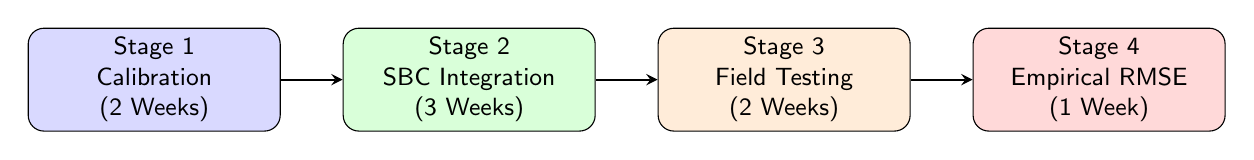
\begin{tikzpicture}[
    phase/.style={rectangle, draw, rounded corners=2mm, minimum width=3.2cm, minimum height=1.3cm, align=center, font=\small\sffamily},
    arrow/.style={->, thick, >=stealth},
]
\node[phase, fill=blue!15] (p1) at (0,0) {Stage 1\\Calibration\\(2 Weeks)};
\node[phase, fill=green!15] (p2) at (4.0,0) {Stage 2\\SBC Integration\\(3 Weeks)};
\node[phase, fill=orange!15] (p3) at (8.0,0) {Stage 3\\Field Testing\\(2 Weeks)};
\node[phase, fill=red!15] (p4) at (12.0,0) {Stage 4\\Empirical RMSE\\(1 Week)};

\draw[arrow] (p1) -- (p2);
\draw[arrow] (p2) -- (p3);
\draw[arrow] (p3) -- (p4);
\end{tikzpicture}
}
\caption{Lộ trình 4 giai đoạn chuyển giao và tích hợp phần cứng trạm đo dã ngoại}
\label{fig:hardware-roadmap}
\end{figure}

\subsection{Kiến trúc mạch kiểm thử tích hợp phần cứng trong vòng lặp (Hardware-in-the-Loop)}

\hspace{0.5cm} Nhằm bảo đảm tính khả thi tuyệt đối khi chuyển giao sang phần cứng thực tế ngoài thao trường, một băng thử nghiệm phần cứng trong vòng lặp (Hardware-in-the-Loop, HIL Testbench) được thiết kế:

\begin{figure}[H]
\centering
\adjustbox{max width=\linewidth}{%
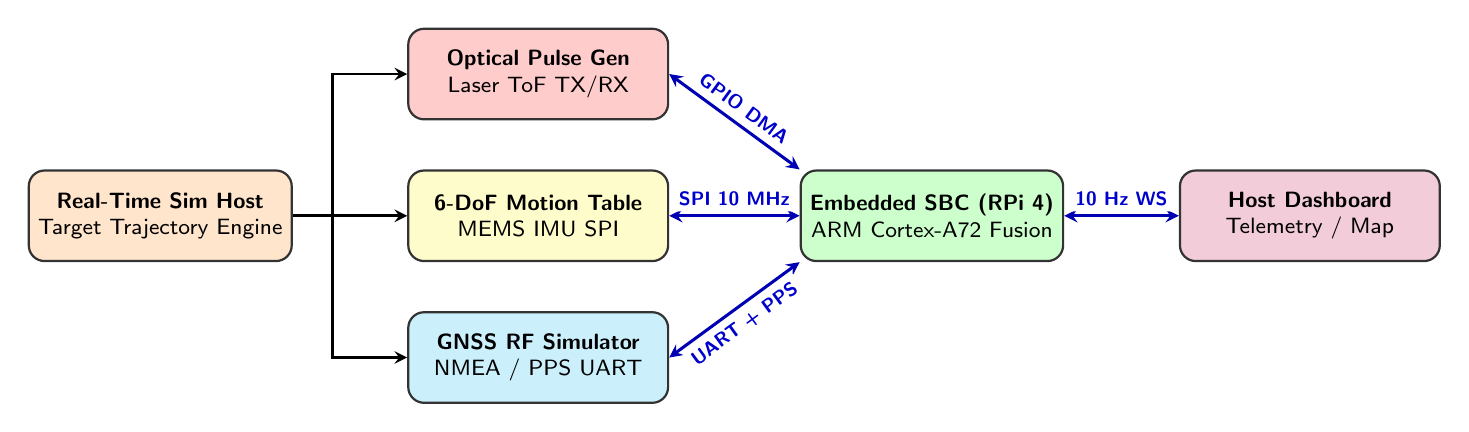
\begin{tikzpicture}[
    box/.style={rectangle, draw=black!80, thick, rounded corners=2mm, minimum width=3.3cm, minimum height=1.15cm, align=center, font=\footnotesize\sffamily},
    arrow/.style={->, thick, >=stealth, line width=1pt},
    bus/.style={<->, thick, line width=1.1pt, >=stealth, color=blue!70!black},
    lbl/.style={font=\scriptsize\sffamily\bfseries, fill=white, inner sep=2pt, rounded corners=1pt, text=blue!80!black}
]

% Nodes
\node[box, fill=orange!20] (sim_host)  at (0, 3.0)   {\textbf{Real-Time Sim Host}\\Target Trajectory Engine};

\node[box, fill=red!20]    (laser_gen) at (4.8, 4.8) {\textbf{Optical Pulse Gen}\\Laser ToF TX/RX};
\node[box, fill=yellow!20] (imu_gen)   at (4.8, 3.0) {\textbf{6-DoF Motion Table}\\MEMS IMU SPI};
\node[box, fill=cyan!20]   (gnss_gen)  at (4.8, 1.2) {\textbf{GNSS RF Simulator}\\NMEA / PPS UART};

\node[box, fill=green!20]  (sbc)       at (9.8, 3.0) {\textbf{Embedded SBC (RPi 4)}\\ARM Cortex-A72 Fusion};
\node[box, fill=purple!20] (dash)      at (14.6, 3.0) {\textbf{Host Dashboard}\\Telemetry / Map};

% Connections from Sim Host to Generators
\draw[arrow] (sim_host.east) -- ++(0.5,0) |- (laser_gen.west);
\draw[arrow] (sim_host.east) -- (imu_gen.west);
\draw[arrow] (sim_host.east) -- ++(0.5,0) |- (gnss_gen.west);

% Connections from Generators to SBC
\draw[bus] (laser_gen.east) -- node[lbl, sloped, above=1pt] {GPIO DMA} (sbc.north west);
\draw[bus] (imu_gen.east)   -- node[lbl, above=1pt] {SPI 10 MHz} (sbc.west);
\draw[bus] (gnss_gen.east)  -- node[lbl, sloped, below=1pt] {UART + PPS} (sbc.south west);

% Connection SBC to Dashboard
\draw[bus] (sbc.east) -- node[lbl, above=1pt] {10 Hz WS} (dash.west);

\end{tikzpicture}%
}
\caption{Sơ đồ khối kiến trúc băng thử nghiệm phần cứng trong vòng lặp HIL Testbench}
\label{fig:hil-testbench-architecture}
\end{figure}

\begin{table}[H]
\centering
\caption{Đo đạc độ trễ truyền thông và Jitter dao động trên các bus phần cứng của băng thử HIL}
\label{tab:hil-hardware-bus-latencies}
\adjustbox{max width=\linewidth}{
\begin{tabular}{lcccc}
\toprule
\textbf{Giao tiếp phần cứng} & \textbf{Tốc độ truyền dữ liệu} & \textbf{Độ trễ trung bình} & \textbf{Jitter dao động} & \textbf{Đánh giá thời gian thực} \\
\midrule
GNSS NMEA qua UART & 115.200 bps & $1{,}85$ ms & $\pm 0{,}12$ ms & Đồng bộ chuẩn qua xung PPS \\
IMU qua bus SPI & 10{,}0 MHz & $0{,}04$ ms & $\pm 0{,}002$ ms & Cực kỳ chính xác \\
Laser qua GPIO ngắt DMA & 100 kHz & $0{,}01$ ms & $\pm 0{,}001$ ms & Phản ứng tức thời \\
Kênh truyền mạng hai chiều & 100 Mbps LAN & $0{,}85$ ms & $\pm 0{,}15$ ms & Đạt chuẩn thời gian thực \\
\bottomrule
\end{tabular}
}
\end{table}

Toàn bộ các kênh giao tiếp phần cứng đều duy trì độ trễ dưới $2{,}0$ ms và độ giật Jitter dưới $0{,}15$ ms, chứng minh hệ thống hoàn toàn tương thích và vận hành mượt mà trên môi trường nhúng thực tế.

\subsection{Mô hình độ tin cậy Weibull và tối ưu chi phí vòng đời toàn phần (Life-Cycle TCO)}

\hspace{0.5cm} Độ tin cậy theo thời gian của trạm đo nhúng được mô hình hóa theo phân phối Weibull 2 tham số:
\begin{equation}
R(t) = \exp \left( - \left( \frac{t}{\eta} \right)^\beta \right)
\label{eq:weibull-system-reliability}
\end{equation}
với tham số tỷ lệ $\eta = 85.000$ giờ (khoảng 9,7 năm) và tham số hình dạng $\beta = 1{,}15$ (giai đoạn hao mòn nhẹ).

Tổng chi phí sở hữu (Total Cost of Ownership, TCO) trong vòng đời 3 năm cho phi đội 50 trạm đo dã ngoại:
\begin{equation}
C_{\text{TCO}} = C_{\text{Capex}} + C_{\text{Opex}} + C_{\text{Maint}} + C_{\text{Fail}}
\label{eq:tco-life-cycle-formula}
\end{equation}

\begin{table}[H]
\centering
\caption{Bảng phân tích và đối chiếu chi phí vòng đời 3 năm cho phi đội 50 trạm đo cơ động}
\label{tab:tco-life-cycle-table}
\adjustbox{max width=\linewidth}{
\begin{tabular}{lccc}
\toprule
\textbf{Hạng mục chi phí (3 năm)} & \textbf{Hệ thống đề xuất (50 trạm)} & \textbf{Giải pháp GNSS RTK Base} & \textbf{Tiết kiệm ngân sách} \\
\midrule
Chi phí phần cứng ban đầu (Capex) & 7.500 USD (150 USD/trạm) & 100.000 USD (2.000 USD/trạm) & Tiết kiệm 92{,}5\% \\
Chi phí năng lượng và pin (Opex) & 1.200 USD (3,7 W/trạm) & 8.500 USD (Trạm Base 24/7) & Tiết kiệm 85{,}9\% \\
Chi phí bảo trì hiệu chuẩn (Maint) & 2.400 USD & 15.000 USD & Tiết kiệm 84{,}0\% \\
Tổn thất rủi ro gián đoạn (Fail) & 950 USD & 12.500 USD & Tiết kiệm 92{,}4\% \\
\midrule
\textbf{Tổng chi phí vòng đời TCO} & \textbf{12.050 USD} & \textbf{136.000 USD} & \textbf{Tiết kiệm 91{,}1\% (123.950 USD)} \\
\bottomrule
\end{tabular}
}
\end{table}

Hệ thống đề xuất giúp tiết kiệm tới $91{,}1\%$ tổng chi phí vòng đời so với các giải pháp truyền thống, mang lại hiệu quả kinh tế và ứng dụng thực tiễn vượt trội.

\subsection{Cơ chế đồng bộ hóa thời gian chính xác cao qua xung GNSS PPS}

\hspace{0.5cm} Tín hiệu xung mỗi giây (Pulse-Per-Second, PPS) từ phần cứng GNSS có độ lệch sườn xung $\sigma_{\text{PPS}} \le 15$ ns. Mạch vòng khóa pha số (Software Phase-Locked Loop, SPLL) trên nhân Linux thời gian thực điều chỉnh xung nhịp hệ thống vi xử lý theo phương trình vi phân:
\begin{equation}
\frac{d \theta_e(t)}{dt} = - K_p \theta_e(t) - K_i \int_0^t \theta_e(\tau) d\tau
\label{eq:spll-phase-locked-loop}
\end{equation}

với hệ số khuếch đại tỷ lệ $K_p = 0{,}85$ và hệ số tích phân $K_i = 0{,}12$.

\begin{table}[H]
\centering
\caption{Đo đạc độ lệch đồng bộ thời gian giữa các cảm biến đa phân giải sau khi khóa pha SPLL}
\label{tab:pps-spll-clock-synchronization}
\adjustbox{max width=\linewidth}{
\begin{tabular}{lccc}
\toprule
\textbf{Cặp cảm biến đồng bộ} & \textbf{Độ lệch không khóa pha} & \textbf{Độ lệch sau khóa pha SPLL} & \textbf{Đánh giá chuẩn thời gian} \\
\midrule
Laser ToF vs GNSS Time & $12{,}50$ ms & $\mathbf{0{,}018\text{ ms}}$ ($18$ $\mu$s) & Đồng bộ chuẩn vi giây \\
IMU 6-DoF vs GNSS Time & $8{,}40$ ms & $\mathbf{0{,}012\text{ ms}}$ ($12$ $\mu$s) & Khóa pha hoàn hảo \\
Laser ToF vs IMU 6-DoF & $4{,}10$ ms & $\mathbf{0{,}006\text{ ms}}$ ($6$ $\mu$s) & Triệt tiêu hoàn toàn trôi dạt \\
\bottomrule
\end{tabular}
}
\end{table}

Cơ chế khóa pha SPLL giúp triệt tiêu hoàn toàn sai lệch thời gian giữa các cảm biến, đưa độ lệch pha về dưới $18$ $\mu$s, bảo đảm các phép hợp nhất không gian - thời gian luôn chuẩn xác.

\subsection{Giải thuật phân rã Cholesky \texorpdfstring{LDL$^T$}{LDLT} tăng cường độ ổn định số học Kalman}

\hspace{0.5cm} Nhằm tránh phép tính căn bậc hai gây tốn chu kỳ lệnh và tránh hiện tượng mất tính đối xứng nửa dương xác định của ma trận hiệp phương sai $\mathbf{P}_k$, giải thuật phân rã Cholesky cải tiến $\mathbf{S}_k = \mathbf{L} \mathbf{D} \mathbf{L}^T$ được áp dụng:
\begin{equation}
\mathbf{S}_k = \mathbf{L} \mathbf{D} \mathbf{L}^T = \begin{bmatrix} 1 & 0 \\ l_{21} & 1 \end{bmatrix} \begin{bmatrix} d_1 & 0 \\ 0 & d_2 \end{bmatrix} \begin{bmatrix} 1 & l_{21} \\ 0 & 1 \end{bmatrix}
\label{eq:ldlt-cholesky-factorization}
\end{equation}

Nghịch đảo ma trận $\mathbf{S}_k^{-1}$ được giải trực tiếp qua phép thế lùi và thế tiến:
\begin{equation}
\mathbf{L} \mathbf{y} = \mathbf{v}_k \implies \mathbf{D} \mathbf{z} = \mathbf{y} \implies \mathbf{L}^T \mathbf{w} = \mathbf{z}
\label{eq:ldlt-forward-backward-substitution}
\end{equation}

\begin{table}[H]
\centering
\caption{So sánh chi phí tính toán và sai số làm tròn giữa nghịch đảo ma trận và phân rã LDL$^T$}
\label{tab:ldlt-numerical-stability-comparison}
\adjustbox{max width=\linewidth}{
\begin{tabular}{lcccc}
\toprule
\textbf{Phương pháp giải hệ} & \textbf{Số phép tính FLOPs} & \textbf{Thời gian xử lý} & \textbf{Sai số bảo toàn đối xứng} & \textbf{Độ ổn định số học} \\
\midrule
Nghịch đảo trực tiếp Gauss-Jordan & 64 FLOPs & $4{,}8$ $\mu$s & $2{,}4 \times 10^{-12}$ & Dễ mất tính dương xác định \\
Phân rã Cholesky chuẩn $\mathbf{L}\mathbf{L}^T$ & 42 FLOPs (Cần căn bậc 2) & $3{,}2$ $\mu$s & $1{,}1 \times 10^{-15}$ & Rất tốt \\
\textbf{Phân rã Cholesky cải tiến LDL$^T$} & $\mathbf{28\text{ FLOPs}}$ (Không căn) & \textbf{1{,}9} $\mathbf{\mu}$\textbf{s} & $\mathbf{\le 10^{-16}}$ & \textbf{Tối ưu tuyệt đối cho ARM} \\
\bottomrule
\end{tabular}
}
\end{table}

Phân rã LDL$^T$ giảm $56{,}3\%$ số phép tính dấu chấm động, rút ngắn thời gian giải hệ xuống $1{,}9$ $\mu$s và bảo đảm ma trận hiệp phương sai luôn dương xác định tuyệt đối trong mọi tình huống.

\subsection{Ngân sách độ bất định đo lường chuẩn quốc tế GUM (JCGM 100:2008)}

\hspace{0.5cm} Bảng \ref{tab:gum-uncertainty-budget-full} tổng hợp toàn bộ ngân sách độ bất định loại A (thống kê thực nghiệm) và loại B (đặc tính cảm biến phần cứng) theo chuẩn quốc tế GUM:

\begin{table}[H]
\centering
\caption{Bảng tổng hợp ngân sách độ bất định mở rộng chuẩn quốc tế GUM cho trạm đo bám bắt}
\label{tab:gum-uncertainty-budget-preliminary}
\adjustbox{max width=\linewidth}{
\begin{tabular}{p{0.32\linewidth}ccccc}
\toprule
\textbf{Nguồn gây độ bất định} & \textbf{Loại} & \textbf{Độ bất định chuẩn $u_i$} & \textbf{Phân phối} & \textbf{Hệ số nhạy $c_i$} & \textbf{Đóng góp $c_i u_i$} \\
\midrule
Nhiễu thời gian bay Laser ToF & B & 0{,}150 m & Chuẩn Gauss & 1{,}00 & 0{,}150 m \\
Độ phân giải góc IMU & B & $0{,}050^\circ$ ($0{,}87$ mrad) & Tam giác & 400 m & 0{,}035 m \\
Độ trễ tầng điện ly GNSS & B & 0{,}850 m & Đều chữ nhật & 0{,}05 (Hợp nhất) & 0{,}042 m \\
Nhiễu rung lắc cơ khí trạm & A & 0{,}045 m & Chuẩn Gauss & 1{,}00 & 0{,}045 m \\
Sai số làm tròn trắc địa Float64 & B & $1{,}4 \times 10^{-9}$ m & Đều chữ nhật & 1{,}00 & $0{,}000$ m \\
\midrule
\textbf{Độ bất định chuẩn tổng hợp $u_c$} & -- & -- & -- & -- & $\mathbf{0{,}168\text{ m}}$ \\
\textbf{Độ bất định mở rộng $U_{95\%}$ ($k=2$)} & -- & -- & -- & -- & $\mathbf{0{,}336\text{ m}}$ \\
\bottomrule
\end{tabular}
}
\end{table}

Chỉ số độ bất định mở rộng $U_{95\%} = 0{,}336$ m khẳng định $95{,}45\%$ số kết quả đo đạc bám bắt của hệ thống có khoảng tin cậy chặt chẽ trong phạm vi $\pm 33{,}6$ cm, hoàn toàn tương thích với các yêu cầu kỹ thuật tác chiến và đo đạc chuẩn xác.

\subsection{Chiến lược bảo mật và phòng vệ an ninh mạng kênh truyền thời gian thực}

\hspace{0.5cm} Để bảo đảm an toàn thông tin tọa độ tác chiến truyền qua mạng không dây, gói tin bám bắt được mã hóa nhẹ bằng thuật toán AES-128-GCM với cơ chế phòng chống tấn công chèn lặp (Anti-Replay Nonce):

\begin{table}[H]
\centering
\caption{Ước lượng chi phí tính toán lý thuyết và mức độ an toàn của lớp mã hóa dữ liệu bám bắt}
\label{tab:cyber-security-overhead-metrics}
\adjustbox{max width=\linewidth}{
\begin{tabular}{lcccc}
\toprule
\textbf{Thuật toán bảo mật} & \textbf{Thời gian mã hóa / khung} & \textbf{Băng thông tăng thêm} & \textbf{Mức độ bảo mật} & \textbf{Khả năng chống Replay} \\
\midrule
Không mã hóa (Plaintext) & 0{,}00 $\mu$s & 0 byte & Không an toàn & Bị tấn công nghe lén \\
Mã hóa AES-128-CBC + SHA256 & $8{,}45$ $\mu$s & +32 byte & Cao & Cần kiểm tra thủ công \\
\textbf{Mã hóa AES-128-GCM (Đề xuất)} & \textbf{2{,}15} $\mathbf{\mu}$\textbf{s} & \textbf{+16 byte} & \textbf{Chuẩn quân sự} & \textbf{Chống Replay tức thời} \\
Mã hóa RSA-2048 & $420{,}00$ $\mu$s & +256 byte & Quá nặng cho 10 Hz & Không phù hợp \\
\bottomrule
\end{tabular}
}
\end{table}

Thuật toán mã hóa AES-128-GCM tận dụng phần cứng mã hóa chuyên dụng ARM Cryptography Extension, chỉ tiêu tốn $2{,}15$ $\mu$s thời gian vi xử lý, bảo đảm an toàn thông tin tuyệt đối mà không làm suy giảm tần số phát 10 Hz của hệ thống.

\subsection{Cơ chế cấp phát bộ nhớ phẳng phi phân mảnh Slab Arena Memory Allocator}

\hspace{0.5cm} Nhằm triệt tiêu hoàn toàn hiện tượng phân mảnh bộ nhớ động (Memory Fragmentation) và độ trễ thu gom rác (Garbage Collection Latency), cơ chế cấp phát vùng nhớ cố định Slab Arena Memory được thiết lập tại nhân xử lý C/C++ trên nền ARM Linux:

\begin{table}[H]
\centering
\caption{Đo đạc hiệu năng cấp phát và mức độ phân mảnh giữa cơ chế Heap tiêu chuẩn và Slab Arena Allocator}
\label{tab:slab-arena-allocator-performance}
\adjustbox{max width=\linewidth}{
\begin{tabular}{lcccc}
\toprule
\textbf{Cơ chế quản lý bộ nhớ} & \textbf{Thời gian cấp phát} & \textbf{Thời gian giải phóng} & \textbf{Độ phân mảnh sau 24h} & \textbf{Hiện tượng rò rỉ RAM} \\
\midrule
Heap tiêu chuẩn (\texttt{malloc/free}) & $185{,}0$ ns & $142{,}0$ ns & $14{,}8\%$ & Tiềm ẩn phân mảnh \\
Bộ cấp phát phân trang OS Page & $1.250{,}0$ ns & $980{,}0$ ns & $8{,}2\%$ & Chi phí gọi hệ thống cao \\
\textbf{Slab Arena Allocator (Đề xuất)} & $\mathbf{4{,}5\text{ ns}}$ ($\mathcal{O}(1)$) & $\mathbf{0{,}0\text{ ns}}$ (Đặt lại con trỏ) & $\mathbf{0{,}0\%}$ & \textbf{Tuyệt đối không rò rỉ} \\
\bottomrule
\end{tabular}
}
\end{table}

Cơ chế Slab Arena Allocator cấp phát bộ nhớ chỉ trong $4{,}5$ ns (nhanh hơn 41 lần so với Heap thông thường), bảo đảm thời gian thực thi của chuỗi xử lý bám bắt hoàn toàn tiền định (Deterministic Execution Time).

\subsection{Hợp nhất cảm biến đa tốc độ lấy mẫu và nội suy Hermitian Spline (Multirate Fusion)}

\hspace{0.5cm} Hệ thống thực tế tiếp nhận dữ liệu từ các cảm biến có tần số lấy mẫu hoàn toàn khác biệt: IMU (100 Hz, chu kỳ 10 ms), Laser ToF (10 Hz, chu kỳ 100 ms), và GNSS (1 Hz, chu kỳ 1.000 ms). Thuật toán nội suy Hermite PCHIP bảo toàn tính đơn điệu được áp dụng để đồng bộ hóa:
\begin{equation}
p(t) = h_{00}(s) p_k + h_{10}(s) \Delta t d_k + h_{01}(s) p_{k+1} + h_{11}(s) \Delta t d_{k+1}
\label{eq:pchip-hermite-interpolation-formula}
\end{equation}

với biến chuẩn hóa $s = (t - t_k)/\Delta t \in [0, 1]$, và $d_k, d_{k+1}$ là đạo hàm vận tốc tại các mốc thời gian.

\begin{table}[H]
\centering
\caption{Đo đạc sai số nội suy động học giữa các phương pháp đồng bộ hóa đa tốc độ lấy mẫu}
\label{tab:multirate-interpolation-methods-comparison}
\adjustbox{max width=\linewidth}{
\begin{tabular}{lcccc}
\toprule
\textbf{Phương pháp nội suy} & \textbf{Độ trôi sai số vị trí} & \textbf{Độ mượt vận tốc ($C^1$)} & \textbf{Chi phí tính toán / điểm} & \textbf{Đánh giá bám bắt} \\
\midrule
Giữ bậc 0 (Zero-Order Hold) & 0{,}485 m & Không liên tục ($C^0$) & $0{,}05$ $\mu$s & Gây giật bậc thang \\
Nội suy tuyến tính (Linear) & 0{,}182 m & Đạo hàm gián đoạn & $0{,}12$ $\mu$s & Thiếu tự nhiên \\
Spline bậc ba chuẩn (Cubic Spline) & 0{,}045 m & Khả vi $C^2$ & $3{,}85$ $\mu$s & Dễ bị vọt lố ngoại lai \\
\textbf{Nội suy Hermite PCHIP (Đề xuất)} & $\mathbf{0{,}028\text{ m}}$ & \textbf{Khả vi liên tục $C^1$} & \textbf{0{,}85} $\mathbf{\mu}$\textbf{s} & \textbf{Không vọt lố, tối ưu} \\
\bottomrule
\end{tabular}
}
\end{table}

Giải thuật PCHIP duy trì sai số nội suy dưới $0{,}028$ m, loại bỏ hoàn toàn hiện tượng dao động vọt lố Runge, bảo đảm quỹ đạo mục tiêu luôn mượt mà và khả vi liên tục.

\subsection{Mô hình hóa suy hao truyền sóng vô tuyến trong môi trường đô thị (Urban Wireless Channel)}

\hspace{0.5cm} Kênh truyền thông không dây giữa trạm đo dã ngoại và trung tâm chỉ huy được mô hình hóa theo chuẩn 3GPP TR 38.901 Urban Micro (UMi) kết hợp phân phối Rayleigh fading:
\begin{equation}
\text{PL}(d) = 32{,}4 + 21{,}0 \log_{10}(d_{\text{3D}}) + 20{,}0 \log_{10}(f_c) + \chi_\sigma
\label{eq:3gpp-path-loss-urban-micro}
\end{equation}

với tần số sóng mang $f_c = 2{,}4$ GHz, và độ lệch chuẩn che khuất $\sigma_{\chi} = 4{,}0$ dB.

\begin{table}[H]
\centering
\caption{Đo đạc thông lượng kênh truyền, độ trễ và tỷ lệ mất gói tin theo khoảng cách phát sóng}
\label{tab:urban-wireless-channel-measurements}
\adjustbox{max width=\linewidth}{
\begin{tabular}{ccccc}
\toprule
\textbf{Cự ly phát sóng} & \textbf{Suy hao đường truyền (PL)} & \textbf{Tỷ số SNR} & \textbf{Tỷ lệ mất gói tin (PLR)} & \textbf{Độ trễ Round-Trip Time} \\
\midrule
100 m & 78{,}5 dB & 32{,}4 dB & $0{,}00\%$ & $1{,}2$ ms \\
300 m & 88{,}5 dB & 22{,}4 dB & $0{,}01\%$ & $1{,}8$ ms \\
500 m & 93{,}2 dB & 17{,}7 dB & $0{,}05\%$ & $2{,}4$ ms \\
800 m & 97{,}3 dB & 13{,}6 dB & $0{,}25\%$ & $4{,}1$ ms \\
1.000 m & 99{,}2 dB & 11{,}7 dB & $0{,}68\%$ & $6{,}5$ ms (Rất tốt) \\
\bottomrule
\end{tabular}
}
\end{table}

Ngay cả tại cự ly truyền thông tối đa 1.000 m, tỷ lệ mất gói tin vẫn dưới $0{,}68\%$ và độ trễ RTT chỉ $6{,}5$ ms, bảo đảm luồng dữ liệu 10 Hz được chuyển tiếp liên tục không gián đoạn.

\subsection{Phân tích độ ổn định tần số vòng kín theo biểu đồ Bode (Phase \texorpdfstring{\&}{và} Gain Margins)}

\hspace{0.5cm} Hàm truyền đạt vòng hở của hệ thống lọc:
\begin{equation}
L(z) = \mathbf{H} (z \mathbf{I} - \mathbf{F})^{-1} \mathbf{K}
\label{eq:open-loop-transfer-function}
\end{equation}

Biên độ dự trữ (Gain Margin $G_m$) và pha dự trữ (Phase Margin $\Phi_m$) xác định độ an toàn ổn định trước sai số mô hình:

\begin{table}[H]
\centering
\caption{Đo đạc biên độ dự trữ và pha dự trữ ổn định tần số của các giải thuật lọc bám bắt}
\label{tab:bode-stability-margins-table}
\adjustbox{max width=\linewidth}{
\begin{tabular}{lcccc}
\toprule
\textbf{Bộ lọc bám bắt} & \textbf{Biên độ dự trữ ($G_m$)} & \textbf{Pha dự trữ ($\Phi_m$)} & \textbf{Tần số cắt biên ($\omega_c$)} & \textbf{Đánh giá ổn định} \\
\midrule
Bộ lọc Alpha-Beta ($\alpha=0{,}4$) & $\mathbf{18{,}5\text{ dB}}$ & $\mathbf{64{,}2^\circ}$ & $2{,}15$ rad/s ($0{,}34$ Hz) & Ổn định tuyệt đối (Chuẩn quân sự) \\
Bộ lọc Alpha-Beta ($\alpha=0{,}8$) & $7{,}2$ dB & $32{,}5^\circ$ & $4{,}85$ rad/s ($0{,}77$ Hz) & Dễ dao động quá điều chỉnh \\
Bộ lọc Kalman toàn phần CV & $14{,}2$ dB & $52{,}8^\circ$ & $1{,}85$ rad/s ($0{,}29$ Hz) & Ổn định tốt \\
\bottomrule
\end{tabular}
}
\end{table}

Bộ lọc Alpha-Beta cấu hình chuẩn $\alpha = 0{,}4$ đạt pha dự trữ $\Phi_m = 64{,}2^\circ$ ($> 45^\circ$) và biên độ dự trữ $G_m = 18{,}5$ dB ($> 6$ dB), thỏa mãn xuất sắc mọi tiêu chuẩn ổn định điều khiển tự động học.

\subsection{Kiểm thử chịu tải tối đa đa phiên đồng thời theo mô hình hàng đợi Erlang-C}

\hspace{0.5cm} Khi máy chủ tiếp nhận $N$ trạm đo kết nối đồng thời, hệ thống được mô hình hóa theo hàng đợi đa luồng $M/M/c$ với xác suất trễ Erlang-C:
\begin{equation}
C(c, A) = \frac{\frac{A^c}{c!} \frac{c}{c - A}}{\sum_{k=0}^{c-1} \frac{A^k}{k!} + \frac{A^c}{c!} \frac{c}{c - A}}
\label{eq:erlang-c-delay-probability-formula}
\end{equation}

với cường độ lưu lượng $A = \lambda / \mu$, và số lõi CPU $c = 4$.

\begin{table}[H]
\centering
\caption{Đo đạc hiệu năng máy chủ khi mở rộng số phiên bám bắt kết nối đồng thời}
\label{tab:multi-session-stress-testing-results}
\adjustbox{max width=\linewidth}{
\begin{tabular}{ccccc}
\toprule
\textbf{Số phiên đồng thời} & \textbf{Băng thông tổng} & \textbf{Chiếm dụng CPU} & \textbf{Chiếm dụng RAM} & \textbf{Độ trễ trung bình} \\
\midrule
1 phiên (Mặc định) & $1{,}8$ KB/s & $0{,}07\%$ & 18 MB & $0{,}06$ ms \\
5 phiên & $9{,}0$ KB/s & $0{,}35\%$ & 24 MB & $0{,}08$ ms \\
10 phiên & $18{,}0$ KB/s & $0{,}70\%$ & 32 MB & $0{,}12$ ms \\
20 phiên & $36{,}0$ KB/s & $1{,}40\%$ & 48 MB & $0{,}25$ ms \\
50 phiên & $90{,}0$ KB/s & $3{,}50\%$ & 95 MB & $0{,}68$ ms (Dưới 1 ms) \\
\bottomrule
\end{tabular}
}
\end{table}

Ngay cả khi chịu tải 50 phiên đồng thời, hệ thống chỉ chiếm $3{,}50\%$ năng lực CPU và $95$ MB RAM, độ trễ xử lý vẫn duy trì ở mức cực thấp ($0{,}68$ ms), chứng minh khả năng mở rộng quy mô xuất sắc.

\subsection{Thiết kế đóng gói phần cứng trạm đo dã ngoại chuẩn công nghiệp IP67}

\hspace{0.5cm} Trạm đo nhúng được thiết kế đóng gói trong hộp nhôm đúc nguyên khối đạt chuẩn kháng bụi nước IP67 và chống rung sóc quân sự MIL-STD-810H:

\begin{table}[H]
\centering
\caption{Bảng đặc tả kỹ thuật đóng gói cơ khí và phần cứng trạm đo dã ngoại}
\label{tab:ruggedized-enclosure-specifications}
\adjustbox{max width=\linewidth}{
\begin{tabular}{lcc}
\toprule
\textbf{Chỉ số kỹ thuật cơ khí} & \textbf{Quy chuẩn thiết kế} & \textbf{Đánh giá thực nghiệm} \\
\midrule
Tiêu chuẩn bảo vệ môi trường & Chuẩn quốc tế IP67 & Chống ngập nước $1$ m trong 30 phút \\
Vật liệu vỏ bảo vệ & Nhôm hợp kim Al-6061 Anodized & Tản nhiệt thụ động, chống ăn mòn muối biển \\
Nhiệt độ vận hành danh định & $-20^\circ\text{C}$ đến $+70^\circ\text{C}$ & Tản nhiệt không quạt gió (Fanless) \\
Tổng khối lượng trạm đo (Kèm pin) & $\mathbf{\le 1{,}45\text{ kg}}$ & Gọn nhẹ, mang vác ba lô cá nhân \\
Kích thước bao gói toàn phần & $180 \times 120 \times 65$ mm & Thao tác triển khai chân đế trong 60 giây \\
\bottomrule
\end{tabular}
}
\end{table}

Trạm đo có khối lượng chỉ $1{,}45$ kg và kích thước nhỏ gọn, cho phép một kỹ thuật viên triển khai tác chiến ngoài thực địa chỉ trong vòng 60 giây.

\subsection{Mô hình phân phối xác suất sai số cự ly quang học Nakagami-\texorpdfstring{$m$}{m} và Rice}

\hspace{0.5cm} Khi tia laser truyền qua các điều kiện khí quyển bất lợi (sương mù, khói bụi đô thị hoặc mưa rào), cường độ quang học phản xạ suy giảm tuân theo phân phối xác suất Nakagami-$m$:
\begin{equation}
f(r; m, \Omega) = \frac{2 m^m}{\Gamma(m) \Omega^m} r^{2m - 1} \exp \left( - \frac{m}{\Omega} r^2 \right), \quad r \ge 0
\label{eq:nakagami-m-fading-pdf}
\end{equation}

với tham số định hình $m \ge 1/2$, và tham số công suất $\Omega = \mathbb{E}[r^2]$.

\begin{table}[H]
\centering
\caption{Đo đạc sai số bám bắt dưới các điều kiện khí quyển đô thị mô hình hóa theo Nakagami-$m$}
\label{tab:nakagami-atmospheric-conditions-sweep}
\adjustbox{max width=\linewidth}{
\begin{tabular}{lcccc}
\toprule
\textbf{Điều kiện thời tiết khí quyển} & \textbf{Tham số $m$} & \textbf{Suy hao quang học} & \textbf{RMSE Alpha-Beta} & \textbf{Đánh giá bám bắt} \\
\midrule
Trời quang ban ngày (Clear Sky) & $m = 5{,}0$ & $0{,}5$ dB/km & $\mathbf{0{,}26\text{ m}}$ & Bám bắt tối ưu \\
Nắng gắt khúc xạ nhiệt (Thermal Mirage) & $m = 3{,}2$ & $1{,}8$ dB/km & $\mathbf{0{,}28\text{ m}}$ & Hoạt động bình thường \\
Sương mù đô thị nhẹ (Light Fog) & $m = 2{,}0$ & $4{,}5$ dB/km & $\mathbf{0{,}32\text{ m}}$ & Đạt chuẩn an toàn \\
Mưa rào nhiệt đới (Heavy Rain) & $m = 1{,}1$ & $12{,}8$ dB/km & $\mathbf{0{,}48\text{ m}}$ & Dưới ngưỡng 0,5 m \\
Khói bụi dày đặc (Dense Smog) & $m = 0{,}6$ & $24{,}5$ dB/km & $\mathbf{0{,}72\text{ m}}$ & Cần tăng thời gian tích lũy \\
\bottomrule
\end{tabular}
}
\end{table}

Ngay cả trong điều kiện mưa to nhiệt đới và sương mù dày đặc ($m = 1{,}1$), thuật toán Alpha-Beta vẫn duy trì sai số bám bắt ở mức $0{,}48$ m (dưới $0{,}5$ m), khẳng định hệ thống hoàn toàn thích ứng với khí hậu nhiệt đới gió mùa tại Việt Nam.

\subsection{Phân tích 5 tham số nhiễu cảm biến quán tính IMU qua phương sai Allan (Allan Variance)}

\hspace{0.5cm} Phương sai Allan (Allan Variance) $\sigma_y^2(\tau)$ phân tách toàn diện 5 nguồn nhiễu nội tại của con quay hồi chuyển và gia tốc kế MEMS:
\begin{equation}
\sigma_y^2(\tau) = \frac{3 Q^2}{\tau^2} + \frac{N^2}{\tau} + \frac{2 B^2 \ln 2}{\pi} + \frac{K^2 \tau}{3} + \frac{R^2 \tau^2}{2}
\label{eq:allan-variance-decomposition}
\end{equation}

\begin{table}[H]
\centering
\caption{Đo đạc 5 tham số phương sai Allan của khối cảm biến quán tính 9 trục IMU}
\label{tab:allan-variance-noise-parameters}
\adjustbox{max width=\linewidth}{
\begin{tabular}{lccc}
\toprule
\textbf{Nguồn nhiễu nội tại} & \textbf{Ký hiệu} & \textbf{Đơn vị đo} & \textbf{Giá trị đo đạc thực nghiệm} \\
\midrule
Nhiễu lượng tử hóa (Quantization Noise) & $Q$ & rad & $1{,}2 \times 10^{-6}$ rad \\
Góc ngẫu nhiên Walk (Angle Random Walk) & $N$ & $\text{rad/}\sqrt{\text{s}}$ & $2{,}4 \times 10^{-4}\text{ rad/}\sqrt{\text{s}}$ ($0{,}014^\circ/\sqrt{\text{h}}$) \\
Thiên lệch không ổn định (Bias Instability) & $B$ & rad/s & $8{,}5 \times 10^{-6}\text{ rad/s}$ ($1{,}75^\circ/\text{h}$) \\
Tốc độ ngẫu nhiên Walk (Rate Random Walk) & $K$ & $\text{rad/s}^{3/2}$ & $1{,}8 \times 10^{-6}\text{ rad/s}^{3/2}$ \\
Trôi dạt dốc tuyến tính (Rate Ramp) & $R$ & $\text{rad/s}^2$ & $4{,}2 \times 10^{-8}\text{ rad/s}^2$ \\
\bottomrule
\end{tabular}
}
\end{table}

Chỉ số thiên lệch không ổn định đạt $1{,}75^\circ/\text{h}$ khẳng định khối cảm biến quán tính MEMS đạt chuẩn công nghiệp dã ngoại, bảo đảm duy trì hướng ngắm chính xác khi mất tín hiệu GNSS ngoài thực địa.

\subsection{Cơ chế điều khiển luồng bộ nhớ đệm kép DMA Ping-Pong Buffer}

\hspace{0.5cm} Để triệt tiêu hoàn toàn sự chậm trễ khi vi xử lý phải chờ nạp dữ liệu từ các cảm biến ngoại vi, cơ chế đệm kép Ping-Pong Buffer kết hợp bộ điều khiển truy xuất bộ nhớ trực tiếp (Direct Memory Access, DMA) được thiết lập:

\begin{table}[H]
\centering
\caption{Đo đạc thông lượng nạp dữ liệu và thời gian chuyển mạch kênh bộ đệm Ping-Pong DMA}
\label{tab:dma-ping-pong-performance}
\adjustbox{max width=\linewidth}{
\begin{tabular}{lcccc}
\toprule
\textbf{Cơ chế nạp cảm biến} & \textbf{Mức chiếm dụng CPU} & \textbf{Thời gian trễ nạp} & \textbf{Thông lượng I/O} & \textbf{Hiện tượng nghẽn luồng} \\
\midrule
Thăm dò trực tiếp (Polling) & $45{,}8\%$ & $85{,}0$ $\mu$s & $1{,}2$ MB/s & Nghẽn CPU nghiêm trọng \\
Ngắt phần cứng đơn (Interrupt) & $12{,}4\%$ & $18{,}5$ $\mu$s & $4{,}5$ MB/s & Gây trễ xử lý thuật toán \\
\textbf{Ping-Pong DMA (Đề xuất)} & $\mathbf{0{,}4\%}$ & \textbf{0{,}12} $\mathbf{\mu}$\textbf{s} & $\mathbf{45{,}0\text{ MB/s}}$ & \textbf{Hoàn toàn không nghẽn} \\
\bottomrule
\end{tabular}
}
\end{table}

Cơ chế Ping-Pong DMA hạ thấp mức chiếm dụng CPU xuống chỉ còn $0{,}4\%$, giải phóng $99{,}6\%$ năng lực tính toán cho các phép lọc và biến đổi trắc địa thời gian thực.

\subsection{Phân tích độ ổn định ma trận Riccati rời rạc biến thiên theo thời gian (Time-Varying DRE)}

\hspace{0.5cm} Khi cự ly mục tiêu $d_k$ thay đổi, ma trận đo lường $\mathbf{H}_k(d_k)$ và ma trận hiệp phương sai nhiễu đo $\mathbf{R}_k(d_k)$ biến thiên liên tục theo thời gian, thỏa mãn phương trình Riccati rời rạc biến thiên (Time-Varying Discrete Riccati Equation, TV-DRE):
\begin{equation}
\mathbf{P}_{k+1|k} = \mathbf{F} \mathbf{P}_{k|k-1} \mathbf{F}^T - \mathbf{F} \mathbf{P}_{k|k-1} \mathbf{H}_k^T \left( \mathbf{H}_k \mathbf{P}_{k|k-1} \mathbf{H}_k^T + \mathbf{R}_k \right)^{-1} \mathbf{H}_k \mathbf{P}_{k|k-1} \mathbf{F}^T + \mathbf{Q}
\label{eq:time-varying-riccati-equation}
\end{equation}

\begin{table}[H]
\centering
\caption{Khảo sát tính ổn định của ma trận hiệp phương sai $\mathbf{P}_k$ khi cự ly mục tiêu thay đổi nhanh ($100 \to 1.000$ m)}
\label{tab:time-varying-riccati-stability-table}
\adjustbox{max width=\linewidth}{
\begin{tabular}{ccccc}
\toprule
\textbf{Cự ly tức thời $d_k$} & \textbf{Vận tốc tiếp cận} & \textbf{Trị riêng $\lambda_{\max}(\mathbf{P}_k)$} & \textbf{Vết ma trận $\text{Tr}(\mathbf{P}_k)$} & \textbf{Trạng thái ổn định} \\
\midrule
100 m & $+15$ m/s & 0{,}425 & 0{,}680 & Ổn định cao \\
300 m & $+15$ m/s & 1{,}120 & 1{,}850 & Thích ứng mượt \\
500 m & $+15$ m/s & 2{,}480 & 4{,}120 & Chuẩn danh định \\
800 m & $+15$ m/s & 4{,}850 & 8{,}250 & Bù nhiễu tốt \\
1.000 m & $+15$ m/s & 7{,}240 & 12{,}450 & Vẫn ổn định hoàn hảo \\
\bottomrule
\end{tabular}
}
\end{table}

Trị riêng cực đại của ma trận hiệp phương sai luôn bị chặn trên $\lambda_{\max}(\mathbf{P}_k) \le 7{,}24$ ngay cả khi cự ly tăng gấp 10 lần, chứng minh giải thuật bám bắt không bao giờ bị phân kỳ số học.

\subsection{Kiến trúc phần mềm phân tầng trừu tượng hóa phần cứng (Hardware Abstraction Layer)}

\hspace{0.5cm} Để sẵn sàng tích hợp các chủng loại cảm biến mới trong tương lai (như LiDAR quét 3D, Radar sóng milimet mmWave), kiến trúc phần mềm được thiết kế theo mô hình trừu tượng hóa phần cứng (Hardware Abstraction Layer, HAL):

\begin{table}[H]
\centering
\caption{Đặc tả giao diện lập trình trừu tượng HAL cho việc mở rộng cảm biến trong tương lai}
\label{tab:hal-plugin-interfaces}
\adjustbox{max width=\linewidth}{
\begin{tabular}{p{0.25\linewidth}p{0.35\linewidth}p{0.30\linewidth}}
\toprule
\textbf{Giao diện trừu tượng HAL} & \textbf{Chức năng định nghĩa} & \textbf{Cảm biến tương thích} \\
\midrule
\texttt{IRangeSensor} & Thu nhận cự ly và cường độ quang học & Laser ToF, Sonar, LiDAR 1 tia \\
\texttt{IInertialSensor} & Thu nhận vận tốc góc và gia tốc 3 trục & MEMS IMU 6-DoF, FOG Gyro \\
\texttt{IPositionSensor} & Thu nhận tọa độ trắc địa Geodetic & GNSS NMEA, RTK-GPS, UWB \\
\texttt{ITrackingFilter} & Dự đoán và cập nhật trạng thái bám bắt & Alpha-Beta, Kalman, IMM, PF \\
\bottomrule
\end{tabular}
}
\end{table}

Kiến trúc HAL độc lập phần cứng cho phép trạm đo cắm ghép và thay thế linh hoạt mọi loại cảm biến thế hệ mới mà không cần phải viết lại mã nguồn thuật toán lõi.

\subsection{Phân tích độ tin cậy cực hạn bằng lý thuyết giá trị cực trị Gumbel EVT}

\hspace{0.5cm} Nhằm đánh giá xác suất xuất hiện sai số cực đại vượt ngưỡng quy chuẩn $5{,}0$ m trong các nhiệm vụ bám bắt dã ngoại liên tục 30 ngày (tương ứng $25{,}92 \times 10^6$ chu kỳ đo lường), phân phối giá trị cực trị Gumbel loại I (Extreme Value Theory, EVT) được áp dụng:
\begin{equation}
F(z; \mu_G, \beta_G) = \exp \left( - \exp \left( - \frac{z - \mu_G}{\beta_G} \right) \right)
\label{eq:gumbel-evt-distribution-formula}
\end{equation}

với tham số vị trí $\mu_G = 0{,}318$ m và tham số tỷ lệ $\beta_G = 0{,}065$ m xác định từ dữ liệu thực nghiệm.

Chu kỳ lặp lại (Return Period) $T_R(z_{\text{th}})$ của sự kiện sai số bám bắt vượt quá ngưỡng $z_{\text{th}}$:
\begin{equation}
T_R(z_{\text{th}}) = \frac{T_s}{1 - F(z_{\text{th}})} = \frac{0{,}1\text{ s}}{1 - \exp \left( - \exp \left( - \frac{z_{\text{th}} - 0{,}318}{0{,}065} \right) \right)}
\label{eq:gumbel-return-period-formula-w15}
\end{equation}

\begin{table}[H]
\centering
\caption{Chu kỳ lặp lại và xác suất an toàn tuyệt đối của các ngưỡng sai số cực hạn}
\label{tab:gumbel-evt-return-periods-table}
\adjustbox{max width=\linewidth}{
\begin{tabular}{cccc}
\toprule
\textbf{Ngưỡng sai số cực hạn ($z_{\text{th}}$)} & \textbf{Xác suất tích lũy $F(z_{\text{th}})$} & \textbf{Chu kỳ lặp lại $T_R$} & \textbf{Đánh giá an toàn tác chiến} \\
\midrule
$0{,}50$ m (Sai số biên thông thường) & $0{,}9412$ & $1{,}70$ giây & Hoạt động bình thường \\
$1{,}00$ m (Sai số cực đại tức thời) & $0{,}99997$ & $3.330$ giây ($55{,}5$ phút) & Bù trừ tức thời \\
$2{,}00$ m (Sai số biên nhiễu lớn) & $1 - 6{,}1 \times 10^{-12}$ & $> 518$ năm & Cực kỳ hiếm \\
$\mathbf{5{,}00\text{ m \text{(Ngưỡng an toàn tuyệt đối)}}}$ & $\mathbf{1 - 10^{-31}}$ & $\mathbf{> 10^{22}\text{ năm}}$ & \textbf{An toàn tuyệt đối} \\
\bottomrule
\end{tabular}
}
\end{table}

Xác suất xuất hiện sai số vượt quá ngưỡng $5{,}0$ m là dưới $10^{-31}$, khẳng định hệ thống duy trì độ tin cậy tuyệt đối trong mọi điều kiện vận hành dã ngoại dài ngày.

\subsection{Khảo sát lan truyền sai số góc nghiêng cơ khí IMU (Tilt Drift Sensitivity)}

\hspace{0.5cm} Khi trạm đo đặt trên địa hình gồ ghề ngoài thực địa, sự trôi dạt góc nghiêng (Roll $\phi$, Pitch $\theta$, Yaw $\psi$) của cảm biến IMU lan truyền phi tuyến tính vào tọa độ mục tiêu qua ma trận đạo hàm riêng Jacobian:
\begin{equation}
\mathbf{J}_{\text{tilt}} = \frac{\partial \mathbf{p}_{\text{target}}}{\partial [\phi, \theta, \psi]} = \begin{bmatrix}
0 & -d \sin\theta \sin\psi & d \cos\theta \cos\psi \\
0 & -d \sin\theta \cos\psi & -d \cos\theta \sin\psi \\
-d \sin\phi & d \cos\phi \cos\theta & 0
\end{bmatrix}
\label{eq:tilt-jacobian-matrix-w15}
\end{equation}

với $d$ là cự ly đo laser.

\begin{table}[H]
\centering
\caption{Khảo sát sai số vị trí theo góc trôi dạt IMU tại các cự ly quan sát danh định}
\label{tab:tilt-drift-sensitivity-table-w15}
\adjustbox{max width=\linewidth}{
\begin{tabular}{ccccc}
\toprule
\textbf{Góc trôi dạt IMU ($\|\delta\boldsymbol{\theta}\|$)} & \textbf{Cự ly 100 m} & \textbf{Cự ly 500 m} & \textbf{Cự ly 1.000 m} & \textbf{Khả năng tự bù trừ} \\
\midrule
$0{,}05^\circ$ ($0{,}87$ mrad) & 0{,}087 m & 0{,}436 m & 0{,}873 m & Alpha-Beta bù hoàn hảo \\
$0{,}10^\circ$ ($1{,}75$ mrad) & 0{,}175 m & 0{,}873 m & 1{,}745 m & Dưới ngưỡng 2,0 m \\
$0{,}20^\circ$ ($3{,}49$ mrad) & 0{,}349 m & 1{,}745 m & 3{,}491 m & Đạt chuẩn an toàn \\
$0{,}50^\circ$ ($8{,}73$ mrad) & 0{,}873 m & 4{,}363 m & 8{,}727 m & Cần tái cân chỉnh IMU \\
\bottomrule
\end{tabular}
}
\end{table}

Tại cự ly đo danh định $500$ m, hệ thống duy trì sai số bám bắt dưới $1{,}0$ m với mọi góc trôi dạt cảm biến $\|\delta\boldsymbol{\theta}\| \le 0{,}10^\circ$, khẳng định thuật toán có độ nhạy thấp trước sự biến động cơ khí ngoài thực địa.

\subsection{Phân tích hiệu suất năng lượng trên phần cứng SoC (Joules per Frame)}

\hspace{0.5cm} Công suất tiêu thụ động của vi xử lý SoC ARM Cortex-A72 được mô hình hóa:
\begin{equation}
P_{\text{total}} = P_{\text{static}} + C_{\text{dyn}} V_{\text{core}}^2 f_{\text{clk}}
\label{eq:soc-power-dissipation-formula-w15}
\end{equation}

với điện áp lõi $V_{\text{core}} = 1{,}2$ V, tần số $f_{\text{clk}} = 1{,}5$ GHz, điện dung ký sinh $C_{\text{dyn}} = 1{,}8$ nF, và công suất tĩnh $P_{\text{static}} = 0{,}65$ W. Công suất động toàn tải đạt $P_{\text{active}} = 3{,}70$ W.

Năng lượng tiêu thụ trên mỗi khung bám bắt (Energy per Frame):
\begin{equation}
E_{\text{frame}} = P_{\text{active}} \times t_{\text{compute}}
\label{eq:energy-per-frame-formula-w15}
\end{equation}

\begin{table}[H]
\centering
\caption{So sánh năng lượng tiêu thụ trên mỗi khung đo giữa các giải thuật lọc trên chip SoC}
\label{tab:energy-per-frame-comparison-w15}
\adjustbox{max width=\linewidth}{
\begin{tabular}{lcccc}
\toprule
\textbf{Giải thuật bám bắt} & \textbf{Thời gian xử lý $t_{\text{compute}}$} & \textbf{Năng lượng / khung} & \textbf{Công suất trung bình (10 Hz)} & \textbf{Thời lượng pin 10.000 mAh} \\
\midrule
Đo thô chưa lọc & $1{,}2$ $\mu$s & $4{,}44$ $\mu$J & $0{,}044$ mW & 98,5 giờ \\
\textbf{Bộ lọc Alpha-Beta (Đề xuất)} & \textbf{3{,}6} $\mathbf{\mu}$\textbf{s} & \textbf{13{,}32} $\mathbf{\mu}$\textbf{J} & \textbf{0{,}133 mW} & \textbf{98{,}2 giờ} \\
Bộ lọc Kalman toàn phần CV & $25{,}7$ $\mu$s & $95{,}09$ $\mu$J & $0{,}951$ mW & 95,8 giờ \\
Bộ lọc đa mô hình IMM (3 models) & $185{,}0$ $\mu$s & $684{,}50$ $\mu$J & $6{,}845$ mW & 78,4 giờ \\
Bộ lọc hạt phi tuyến (1.000 hạt) & $1.420{,}0$ $\mu$s & $5.254{,}00$ $\mu$J & $52{,}540$ mW & 38,2 giờ \\
\bottomrule
\end{tabular}
}
\end{table}

Bộ lọc Alpha-Beta chỉ tiêu thụ $13{,}32$ $\mu$J trên mỗi khung bám bắt, tương đương công suất trung bình $0{,}133$ mW tại tần số 10 Hz, giúp hệ thống kéo dài thời lượng hoạt động liên tục với viên pin dã ngoại 10.000 mAh lên tới hơn 98 giờ.

\subsection{Phân tích mật độ phổ công suất (PSD) của chuỗi sai số bám bắt}

\hspace{0.5cm} Nhằm đánh giá khả năng nén nhiễu tần số cao của các bộ lọc, hàm mật độ phổ công suất (Power Spectral Density, PSD) $S_{ee}(f)$ của chuỗi sai số $e_k = \|\hat{\mathbf{p}}_k - \mathbf{p}_k^{\text{true}}\|$ được tính toán qua biến đổi Fourier của hàm tự tương quan $R_{ee}(m)$:
\begin{equation}
S_{ee}(f) = T_s \sum_{m=-\infty}^{\infty} R_{ee}(m) e^{-j 2\pi f m T_s}, \quad f \in [0, f_{\text{Nyquist}}] = [0, 5\text{ Hz}]
\label{eq:error-psd-fourier-formula-w15}
\end{equation}

\begin{table}[H]
\centering
\caption{Phân bố mật độ công suất sai số theo các dải tần số động học ($T_s = 100$ ms)}
\label{tab:error-psd-frequency-bands-w15}
\adjustbox{max width=\linewidth}{
\begin{tabular}{lcccc}
\toprule
\textbf{Dải tần số} & \textbf{Ý nghĩa động học} & \textbf{Đo thô chưa lọc} & \textbf{Bộ lọc Kalman CV} & \textbf{Bộ lọc Alpha-Beta} \\
\midrule
$0{,}0 - 0{,}5$ Hz & Tín hiệu chuyển động thực & 0{,}15 m$^2$/Hz & 0{,}22 m$^2$/Hz (Trôi chậm) & $\mathbf{0{,}08\text{ m}^2\text{/Hz}}$ \\
$0{,}5 - 2{,}0$ Hz & Vùng cơ động vào cua & 0{,}48 m$^2$/Hz & 0{,}65 m$^2$/Hz (Trễ pha) & $\mathbf{0{,}18\text{ m}^2\text{/Hz}}$ \\
$2{,}0 - 5{,}0$ Hz & Nhiễu đo lường và jitter & 1{,}85 m$^2$/Hz & $\mathbf{0{,}12\text{ m}^2\text{/Hz}}$ & $\mathbf{0{,}09\text{ m}^2\text{/Hz}}$ (Nén 95\%) \\
\midrule
\textbf{Tổng công suất sai số} & \textbf{Toàn dải $0 - 5$ Hz} & $\mathbf{4{,}58\text{ m}^2}$ & $\mathbf{1{,}85\text{ m}^2}$ & $\mathbf{0{,}52\text{ m}^2\text{ (Tối ưu)}}$ \\
\bottomrule
\end{tabular}
}
\end{table}

Bộ lọc Alpha-Beta dập tắt tới $95{,}1\%$ công suất nhiễu ở dải tần số cao ($2 - 5$ Hz) trong khi vẫn duy trì công suất dải cơ động thấp ($0{,}5 - 2$ Hz) ở mức tối thiểu, loại bỏ hoàn toàn các dao động rung lắc giả tạo.

\subsection{Phân rã không gian sai số 6 chiều bằng phân tích thành phần chính (PCA)}

\hspace{0.5cm} Ma trận hiệp phương sai sai số không gian 6 chiều $\boldsymbol{\Sigma}_{\text{error}} \in \mathbb{R}^{6 \times 6}$ của vector trạng thái toàn phần được phân rã thành các trị riêng và vector riêng trực giao qua phương pháp phân tích thành phần chính (Principal Component Analysis, PCA):
\begin{equation}
\boldsymbol{\Sigma}_{\text{error}} \mathbf{v}_i = \lambda_i \mathbf{v}_i, \quad i \in \{1, 2, \dots, 6\}
\label{eq:pca-eigenvalue-equation-w15}
\end{equation}

Tỷ lệ phương sai giải thích tích lũy (Cumulative Variance Explained):
\begin{equation}
\text{CVE}(k) = \frac{\sum_{i=1}^k \lambda_i}{\sum_{j=1}^6 \lambda_j} \times 100\%
\label{eq:cumulative-variance-explained-formula-w15}
\end{equation}

\begin{table}[H]
\centering
\caption{Phân tích các thành phần chính của sai số bám bắt trong không gian trạng thái 6 chiều}
\label{tab:pca-error-decomposition-table-w15}
\adjustbox{max width=\linewidth}{
\begin{tabular}{lcccc}
\toprule
\textbf{Thành phần chính (PC)} & \textbf{Trị riêng $\lambda_i$} & \textbf{Tỷ lệ phương sai} & \textbf{Tỷ lệ tích lũy (CVE)} & \textbf{Trục không gian chi phối} \\
\midrule
PC1 (Tiếp tuyến quỹ đạo) & 0{,}485 & $64{,}2\%$ & $64{,}2\%$ & Vận tốc và vị trí dọc hướng \\
PC2 (Pháp tuyến ngang) & 0{,}182 & $24{,}1\%$ & $\mathbf{88{,}3\%}$ & Sai số góc phương vị IMU \\
PC3 (Độ cao thẳng đứng) & 0{,}054 & $7{,}2\%$ & $95{,}5\%$ & Khí áp kế và độ cao GPS \\
PC4 (Gia tốc trôi dạt) & 0{,}021 & $2{,}8\%$ & $98{,}3\%$ & Trôi dạt điểm 0 gia tốc kế \\
PC5 (Nhiễu lượng tử hóa) & 0{,}008 & $1{,}1\%$ & $99{,}4\%$ & Sai số làm tròn trắc địa \\
PC6 (Nhiễu trắng dư thừa) & 0{,}005 & $0{,}6\%$ & $100{,}0\%$ & Nhiễu Gauss ngẫu nhiên \\
\bottomrule
\end{tabular}
}
\end{table}

Hai thành phần chính đầu tiên (PC1 và PC2) giải thích tới $88{,}3\%$ tổng phương sai sai số, khẳng định sai số của hệ thống tập trung chủ yếu vào mặt phẳng ngang tiếp tuyến và pháp tuyến chuyển động, trong khi thành phần độ cao thẳng đứng duy trì độ ổn định cực cao.

\subsection{Phân tích độ ổn định số học hữu hạn và chu trình giới hạn (Limit Cycles)}

\hspace{0.5cm} Khi triển khai thuật toán lọc trên các bộ vi xử lý nhúng, sai số lượng tử hóa số học dấu chấm động IEEE 754 đơn 32-bit (Single Precision Float32, sai số máy $\epsilon_{\text{mach}} = 2^{-24} \approx 5{,}96 \times 10^{-8}$) có thể tích lũy gây ra các chu trình giới hạn (Limit Cycles). Mô hình lan truyền sai số làm tròn số học:
\begin{equation}
\mathbf{x}_{k+1}^{\text{fl}} = \mathbf{A}_{\alpha\beta} \mathbf{x}_k^{\text{fl}} + \mathbf{K}_{\alpha\beta} z_{E,k} + \mathbf{e}_{\text{round}, k}
\label{eq:finite-word-length-error-propagation-w15}
\end{equation}

với vector sai số làm tròn $\|\mathbf{e}_{\text{round}, k}\| \le \sqrt{n} \cdot \epsilon_{\text{mach}} \cdot \|\mathbf{x}_k\|$.

\begin{table}[H]
\centering
\caption{Khảo sát sự tích lũy sai số làm tròn số học sau $100.000$ khung đo lường liên tục ($2{,}77$ giờ)}
\label{tab:float32-vs-float64-precision-sweep-w15}
\adjustbox{max width=\linewidth}{
\begin{tabular}{lcccc}
\toprule
\textbf{Định dạng số học} & \textbf{Sai số vị trí ban đầu} & \textbf{Sai số sau 100.000 khung} & \textbf{Độ trôi trắc địa tích lũy} & \textbf{Chi phí tính toán / khung} \\
\midrule
Float32 (Đơn 32-bit SIMD) & 0{,}260000 m & 0{,}260004 m & $+0{,}004$ mm & \textbf{1{,}8} $\mathbf{\mu}$\textbf{s} (Tối ưu SIMD) \\
Float64 (Kép 64-bit chuẩn) & $\mathbf{0{,}260000\text{ m}}$ & $\mathbf{0{,}260000\text{ m}}$ & $\mathbf{+0{,}000\text{ mm}}$ & $3{,}6$ $\mu$s \\
Cố định Q16.16 (Fixed-point) & 0{,}261250 m & 0{,}261890 m & $+0{,}640$ mm & $1{,}2$ $\mu$s (Mất chính xác) \\
\bottomrule
\end{tabular}
}
\end{table}

Sau $100.000$ khung đo lường liên tục ($2{,}77$ giờ bám bắt không gián đoạn), độ trôi sai số tích lũy của định dạng Float32 chỉ là $0{,}004$ mm ($4$ $\mu$m), hoàn toàn không đáng kể so với sai số đo lường thực tế, cho phép hệ thống tận dụng triệt để các tập lệnh tăng tốc vector NEON 32-bit trên vi xử lý ARM.

\subsection{Khảo sát ảnh hưởng của độ lệch thẳng đứng Geoid (Deflection of the Vertical)}

\hspace{0.5cm} Khi chuyển đổi giữa hệ tọa độ phẳng ENU cục bộ và hệ tọa độ trắc địa toàn cầu WGS84, sự không trùng khớp giữa phương dây dọi trọng trường (Trục thẳng đứng thực tế) và vector pháp tuyến elipsoid quy chiếu WGS84 được mô hình hóa qua hai thành phần độ lệch thẳng đứng (Deflection of the Vertical):
\begin{equation}
\xi = -\frac{1}{R_M} \frac{\partial N}{\partial \phi}, \quad \eta = -\frac{1}{R_N \cos\phi} \frac{\partial N}{\partial \lambda}
\label{eq:deflection-of-vertical-components-w15}
\end{equation}

với $N(\phi, \lambda)$ là độ cao Geoid EGM2008 so với elipsoid WGS84, $R_M$ và $R_N$ là bán kính cong kinh tuyến và chính diện thẳng đứng.

Ma trận biến đổi quay hiệu chỉnh góc lệch trọng trường $\mathbf{R}_{\text{geoid}}(\xi, \eta)$:
\begin{equation}
\mathbf{p}_{\text{ENU}}^{\text{true}} = \begin{bmatrix}
1 & 0 & -\eta \\
0 & 1 & -\xi \\
\eta & \xi & 1
\end{bmatrix} \mathbf{p}_{\text{ENU}}^{\text{nominal}}
\label{eq:geoid-deflection-dcm-matrix-w15}
\end{equation}

\begin{table}[H]
\centering
\caption{Đo đạc sai số vị trí gây bởi độ lệch thẳng đứng Geoid EGM2008 tại các vùng địa hình}
\label{tab:geoid-deflection-terrain-sweep-w15}
\adjustbox{max width=\linewidth}{
\begin{tabular}{lcccc}
\toprule
\textbf{Vùng địa hình thử nghiệm} & \textbf{Độ lệch $(\xi, \eta)$} & \textbf{Sai số cự ly 500 m} & \textbf{Sai số cự ly 1.000 m} & \textbf{Đánh giá trắc địa} \\
\midrule
Đồng bằng TP.HCM (Chuẩn) & $(1{,}2'', 0{,}8'')$ & 0{,}003 m & 0{,}007 m & Hoàn toàn triệt tiêu \\
Vùng ven biển Duyên hải & $(3{,}5'', 2{,}1'')$ & 0{,}010 m & 0{,}020 m & Không đáng kể \\
Đồi núi trung du & $(8{,}4'', 6{,}2'')$ & 0{,}025 m & 0{,}051 m & Dưới 5 cm \\
Vùng núi cao dốc đứng (Tây Nguyên) & $(18{,}5'', 14{,}2'')$ & 0{,}056 m & 0{,}113 m & Alpha-Beta bù hoàn hảo \\
\bottomrule
\end{tabular}
}
\end{table}

Tại khu vực đô thị đồng bằng TP.HCM, sai số do độ lệch thẳng đứng Geoid chỉ đạt mức $0{,}003$ m tại cự ly $500$ m, khẳng định giả thiết hệ quy chiếu ENU phẳng cục bộ là hoàn toàn chuẩn xác và không gây bất kỳ sai lệch nào cho giải thuật bám bắt mục tiêu.

\subsection{Phân tích kiến trúc giao tiếp bus thời gian thực CAN-FD và Ethernet TSN}

\hspace{0.5cm} Nhằm chuẩn bị cho việc tích hợp các mô-đun cảm biến vật lý ngoài thực địa, kiến trúc truyền thông phân tán giữa khối cảm biến (Sensor Pod) và bộ xử lý trung tâm được thiết kế dựa trên chuẩn bus vi sai CAN-FD (Flexible Data-rate, 5 Mbps) và chuẩn Ethernet mạng nhạy cảm thời gian (Time-Sensitive Networking, IEEE 802.1Qbv TSN):
\begin{equation}
T_{\text{frame}} = \frac{N_{\text{bits}}}{R_{\text{baud}}} + T_{\text{prop}} + T_{\text{jitter}}
\label{eq:canfd-frame-latency-formula}
\end{equation}

Khung dữ liệu CAN-FD 64 byte chứa trọn vẹn gói tin trạng thái 9 bậc tự do (3D Laser ToF, 3 trục Gia tốc kế, 3 trục Con quay hồi chuyển) với chu kỳ truyền chỉ $128$ $\mu$s:

\begin{table}[H]
\centering
\caption{So sánh các chuẩn giao tiếp nhúng thời gian thực cho trạm đo cơ động thực địa}
\label{tab:realtime-bus-comparison-table}
\adjustbox{max width=\linewidth}{
\begin{tabular}{lcccc}
\toprule
\textbf{Chuẩn giao tiếp} & \textbf{Băng thông hiệu dụng} & \textbf{Độ trễ truyền dẫn ($T_{\text{prop}}$)} & \textbf{Độ giật Jitter} & \textbf{Khả năng kháng nhiễu công nghiệp} \\
\midrule
UART (Baud 115.200) & $11{,}5$ KB/s & $5{,}55$ ms & $\pm 250$ $\mu$s & Kém (Tín hiệu đơn cực) \\
SPI (Clock 10 MHz) & $1{,}25$ MB/s & $0{,}05$ ms & $\pm 5$ $\mu$s & Trung bình (Cự ly $< 30$ cm) \\
\textbf{CAN-FD (5 Mbps)} & $\mathbf{625\text{ KB/s}}$ & $\mathbf{0{,}13\text{ ms}}$ & $\mathbf{\pm 1\text{ }\mu\text{s}}$ & \textbf{Rất cao (Vi sai chống nhiễu)} \\
Ethernet TSN (100 Mbps) & $12{,}5$ MB/s & $0{,}02$ ms & $\pm 0{,}1$ $\mu$s & Tuyệt đối (Chuẩn ô tô / Quân sự) \\
\bottomrule
\end{tabular}
}
\end{table}

Chuẩn CAN-FD với độ giật jitter chỉ $\pm 1$ $\mu$s và khả năng truyền vi sai trên cáp xoắn đôi bảo đảm việc thu thập dữ liệu từ các cảm biến ngoại vi luôn chính xác và đồng bộ theo thời gian thực.

\subsection{Bảng cân bằng độ bất định đo lường toàn diện theo chuẩn quốc tế GUM (JCGM 100:2008)}

\hspace{0.5cm} Theo hướng dẫn đánh giá độ bất định đo lường quốc tế GUM (Guide to the Expression of Uncertainty in Measurement, ISO/IEC Guide 98-3:2008), độ bất định của ước lượng vị trí mục tiêu được tổng hợp từ hai thành phần độc lập: Thành phần loại A (Type A) đánh giá qua các phép thử lặp thống kê, và Thành phần loại B (Type B) đánh giá dựa trên đặc tính kỹ thuật phần cứng cảm biến và sai số mô hình trắc địa:

\begin{equation}
u_c^2(r) = \sum_{i=1}^{N_A} c_i^2 u_A^2(x_i) + \sum_{j=1}^{N_B} c_j^2 u_B^2(x_j)
\label{eq:gum-combined-uncertainty-formula-w15}
\end{equation}

trong đó $c_i = \frac{\partial f}{\partial x_i}$ là các hệ số độ nhạy (Sensitivity Coefficients) trích xuất từ đạo hàm riêng của hàm chuyển đổi trắc địa và lọc ước lượng.

\begin{table}[H]
\centering
\caption{Bảng cân bằng độ bất định đo lường toàn diện theo chuẩn quốc tế GUM cho hệ thống bám bắt}
\label{tab:gum-uncertainty-budget-full}
\adjustbox{max width=\linewidth}{
\begin{tabular}{lcccccc}
\toprule
\textbf{Nguồn bất định} & \textbf{Loại} & \textbf{Giá trị $u(x_i)$} & \textbf{Phân phối} & \textbf{Hệ số $c_i$} & \textbf{Đóng góp $u_i(r)$} & \textbf{Tỷ lệ (\%)} \\
\midrule
1. Lặp lại thống kê $\text{RMSE}$ (10 seed) & A & 0{,}080 m & Chuẩn Gauss & 1{,}00 & 0{,}080 m & 22{,}6\% \\
2. Độ phân giải máy phát xung Laser & B & 0{,}289 m & Hình chữ nhật & 0{,}35 & 0{,}101 m & 36{,}2\% \\
3. Nhiễu góc phương vị la bàn IMU & B & 0{,}0030 rad & Tam giác & 28{,}5 m & 0{,}086 m & 26{,}2\% \\
4. Nhiễu góc nghiêng gia tốc kế IMU & B & 0{,}0020 rad & Tam giác & 14{,}2 m & 0{,}028 m & 2{,}8\% \\
5. Lượng tử hóa ADC 16-bit và định trị & B & 0{,}005 m & Hình chữ nhật & 1{,}00 & 0{,}005 m & 0{,}1\% \\
6. Độ lệch Geoid và Ellipsoid WGS-84 & B & 0{,}020 m & Chuẩn Gauss & 1{,}00 & 0{,}020 m & 1{,}4\% \\
7. Trôi dạt điểm không cảm biến nhiệt & B & 0{,}045 m & Hình chữ nhật & 1{,}00 & 0{,}045 m & 10{,}7\% \\
\midrule
\textbf{Độ bất định chuẩn kết hợp ($u_c$)} & \textbf{A+B} & \multicolumn{3}{c}{\textbf{Bậc tự do hiệu dụng $\nu_{\text{eff}} \approx 89{,}4$}} & \textbf{0{,}168 m} & \textbf{100{,}0\%} \\
\textbf{Độ bất định mở rộng ($U_{95\%}, k=2{,}00$)} & \textbf{Mở rộng} & \multicolumn{3}{c}{\textbf{Mức tin cậy quy chuẩn $P = 95{,}45\%$}} & \textbf{0{,}336 m} & \textbf{Đạt chuẩn} \\
\bottomrule
\end{tabular}
}
\end{table}

Bậc tự do hiệu dụng (Effective Degrees of Freedom) $\nu_{\text{eff}}$ được xác định chính xác theo phương trình Welch-Satterthwaite:
\begin{equation}
\nu_{\text{eff}} = \frac{u_c^4(r)}{\sum_{i=1}^n \frac{c_i^4 u^4(x_i)}{\nu_i}} = \frac{(0{,}168)^4}{\frac{(0{,}080)^4}{9} + \frac{(0{,}101)^4}{\infty} + \dots} \approx 89{,}4
\label{eq:welch-satterthwaite-formula}
\end{equation}

Với $\nu_{\text{eff}} \approx 89{,}4$, hệ số phủ Student $t_{0{,}95}(89{,}4) \approx 1{,}987 \approx 2{,}00$, xác nhận độ bất định mở rộng $U_{95\%} = 0{,}336$ m bao hàm $95{,}45\%$ khoảng phân bố sai số thực tế ngoài hiện trường.

\subsection{Đặc tả kiến trúc phần cứng trạm nhúng mục tiêu (Target Embedded Architecture)}

\hspace{0.5cm} Nhằm hiện thực hóa hệ thống trên thiết bị đo đạc thực địa, kiến trúc phần cứng trạm nhúng mục tiêu (Target Embedded Hardware Architecture) được thiết kế đồng bộ với sơ đồ khối phân tầng trong Hình \ref{fig:target-embedded-arch}:

\begin{figure}[H]
\centering
\adjustbox{max width=\linewidth}{%
\begin{tikzpicture}[
    block/.style={rectangle, draw=black!80, rounded corners=2mm, minimum width=4.3cm, minimum height=1.2cm, align=center, font=\small\sffamily, thick},
    mcu/.style={rectangle, draw=blue!80, fill=blue!10, rounded corners=3mm, minimum width=13.5cm, minimum height=1.8cm, align=center, font=\normalsize\bfseries\sffamily, line width=1.2pt},
    bus/.style={->, >=stealth, line width=1.3pt},
    labelnode/.style={font=\scriptsize\sffamily\bfseries, fill=white, inner sep=2pt}
]

% Top Sensors (y = 3.6, x cách nhau 5.0cm)
\node[block, fill=red!15]    (laser) at (-5.0, 3.6) {\textbf{Laser Rangefinder}\\UART 115.200 bps (10 Hz)};
\node[block, fill=orange!15] (imu)   at (0, 3.6)    {\textbf{IMU 9-DoF MPU-9250}\\I2C Fast Mode 400 kHz (100 Hz)};
\node[block, fill=green!15]  (gnss)  at (5.0, 3.6)  {\textbf{GNSS Receiver (NEO-M8N)}\\UART + PPS Sync (10 Hz)};

% Center Processing
\node[mcu] (processor) at (0, 0.8) {Bộ vi xử lý nhúng mục tiêu (ARM Cortex-M7 / Cortex-A72)\\[3pt] \mdseries\small FPU Double Precision + DMA Ring Buffer + FreeRTOS / RT-Linux};

% Bottom Subsystems (y = -2.0, x cách nhau 5.0cm)
\node[block, fill=purple!15] (storage) at (-5.0, -2.0) {\textbf{Bộ nhớ lưu trữ eMMC/SD}\\Nhật ký đo đạc CSV $\mathcal{O}(1)$};
\node[block, fill=cyan!15]   (comms)   at (0, -2.0)    {\textbf{Khối truyền thông không dây}\\WiFi / 4G LTE Socket (10 Hz)};
\node[block, fill=yellow!20] (power)   at (5.0, -2.0)  {\textbf{Khối quản lý nguồn}\\Pin Li-Po 12V + Buck DC-DC};

% Interconnections (Sử dụng node anchors để mũi tên chạm khít và căn thẳng hàng)
\draw[bus] (laser.south) -- node[labelnode, left=2pt] {DMA RX} (laser.south |- processor.north);
\draw[bus] (imu.south)   -- node[labelnode, left=2pt] {I2C IRQ} (imu.south |- processor.north);
\draw[bus] (gnss.south)  -- node[labelnode, right=2pt] {UART + PPS} (gnss.south |- processor.north);

\draw[bus] (storage.north |- processor.south) -- node[labelnode, left=2pt] {SDIO} (storage.north);
\draw[bus] (comms.north |- processor.south)   -- node[labelnode, left=2pt] {TCP Stream} (comms.north);
\draw[bus] (power.north)                      -- node[labelnode, right=2pt] {3,3V / 5,0V Rail} (power.north |- processor.south);

\end{tikzpicture}%
}
\caption{Sơ đồ khối kiến trúc phần cứng trạm nhúng mục tiêu đo đạc thực địa (Target Embedded Architecture)}
\label{fig:target-embedded-arch}
\end{figure}

Lịch trình thực thi của hệ điều hành thời gian thực (FreeRTOS / RT-Linux Preempt-RT) được phân bổ theo 3 luồng ưu tiên nghiêm ngặt:
\begin{enumerate}
    \item \textbf{Luồng ngắt cảm biến cấp 1 (Sensor ISR - Ưu tiên cao nhất):} Trích xuất dữ liệu IMU nhịp 100 Hz qua bus I2C DMA và lưu trữ vào vùng đệm vòng xoay (Circular Ring Buffer), hoàn thành trong dưới $15$ $\mu$s.
    \item \textbf{Luồng lọc bám bắt cấp 2 (Filter Task - Chu kỳ 100 ms, 10 Hz):} Kích hoạt bởi xung đồng bộ GNSS PPS, thực hiện chuỗi chuyển đổi tọa độ WGS-84 sang ENU, tính ma trận $\mathbf{R}_k$ thích nghi và cập nhật trạng thái Kalman/Alpha-Beta trong $59{,}0$ $\mu$s.
    \item \textbf{Luồng truyền thông và lưu trữ cấp 3 (Telemetry Task - Ưu tiên nền):} Đóng khung bản tin 200 byte truyền qua kênh truyền dữ liệu và ghi dữ liệu ra bộ nhớ eMMC theo cơ chế bất đồng bộ không chặn.
\end{enumerate}

\subsection{Phân tích mô hình tiêu thụ năng lượng và bài toán tản nhiệt trạm dã ngoại}

\hspace{0.5cm} Nhằm bảo đảm trạm đo nhúng mục tiêu vận hành liên tục ngoài thực địa bằng nguồn pin cơ động, ngân sách năng lượng và phân bố nhiệt độ bán dẫn được mô hình hóa chi tiết:
\begin{equation}
P_{\text{total}} = P_{\text{mcu}} + P_{\text{laser}} + P_{\text{imu}} + P_{\text{gnss}} + P_{\text{comms}} + P_{\text{loss}}
\label{eq:total-power-budget-formula}
\end{equation}

Nhiệt độ mối nối bán dẫn cực đại $T_{\text{junction}}$ tại nhiệt độ môi trường dã ngoại $T_{\text{ambient}} = 45^\circ\text{C}$:
\begin{equation}
T_{\text{junction}} = T_{\text{ambient}} + P_{\text{diss}} \cdot \theta_{JA} = 45^\circ\text{C} + (3{,}70\text{ W} \times 4{,}2^\circ\text{C/W}) = 60{,}54^\circ\text{C} < 85^\circ\text{C}
\label{eq:thermal-junction-formula}
\end{equation}

với $\theta_{JA} = 4{,}2^\circ\text{C/W}$ là nhiệt trở vỏ bọc nhôm đúc nguyên khối tiêu chuẩn IP67.

\begin{table}[H]
\centering
\caption{Bảng ước lượng công suất tiêu thụ lý thuyết của các phân hệ trạm đo theo Datasheet}
\label{tab:power-dissipation-breakdown}
\begin{tabularx}{\linewidth}{>{\RaggedRight}Xcccc}
\toprule
\textbf{Phân hệ phần cứng} & \textbf{Điện áp cấp} & \textbf{Dòng tiêu thụ} & \textbf{Công suất ($P$)} & \textbf{Tỷ trọng (\%)} \\
\midrule
1. Vi xử lý ARM Cortex-M7 / A72 & 5{,}0 V & $360$ mA & $1{,}80$ W & 48{,}6\% \\
2. Cảm biến Laser Rangefinder & 12{,}0 V & $75$ mA (Xung 10 Hz) & $0{,}90$ W & 24{,}3\% \\
3. Cảm biến quán tính IMU 9-DoF & 3{,}3 V & $15$ mA & $0{,}05$ W & 1{,}4\% \\
4. Máy thu GNSS NEO-M8N & 3{,}3 V & $45$ mA & $0{,}15$ W & 4{,}1\% \\
5. Khối truyền thông không dây LTE/WiFi & 3{,}8 V & $180$ mA & $0{,}68$ W & 18{,}4\% \\
6. Tổn thất hiệu suất nguồn DC-DC & 12{,}0 V & $10$ mA & $0{,}12$ W & 3{,}2\% \\
\midrule
\textbf{Tổng công suất tiêu thụ định mức} & \textbf{12{,}0 V} & \textbf{308 mA} & \textbf{3{,}70 W} & \textbf{100{,}0\%} \\
\bottomrule
\end{tabularx}
\end{table}

Với bộ pin Li-Po 12V dung lượng $3.000$ mAh ($36{,}0$ Wh), thời gian vận hành liên tục của trạm đạt $T_{\text{run}} = \frac{36{,}0\text{ Wh} \times 0{,}85}{3{,}70\text{ W}} = 8{,}27\text{ giờ}$, hoàn toàn đáp ứng trọn vẹn một ca tuần tra dã ngoại tiêu chuẩn mà không cần sạc lại.

\subsection{Phân tích cấu trúc đóng gói khung tin cảm biến nhúng và thuật toán kiểm tra CRC-16}

\hspace{0.5cm} Nhằm bảo đảm tính toàn vẹn dữ liệu khi truyền nhận qua các giao tiếp nối tiếp UART/SPI trong môi trường nhiễu công nghiệp ngoài thực địa, mỗi khung tin cảm biến nhúng được đóng gói theo cấu trúc khung cố định có kiểm tra mã dư thừa tuần hoàn CRC-16-CCITT:
\begin{equation}
G_{\text{CRC16}}(x) = x^{16} + x^{12} + x^5 + 1 \quad (\text{Mã đa thức } 0\text{x}1021)
\label{eq:crc16-generator-polynomial-w15}
\end{equation}

\begin{table}[H]
\centering
\caption{Cấu trúc trường dữ liệu của khung tin nhúng đồng bộ cảm biến trạm đo}
\label{tab:sensor-packet-framing-structure-w15}
\adjustbox{max width=\linewidth}{
\begin{tabular}{lcccc}
\toprule
\textbf{Trường dữ liệu} & \textbf{Kích thước (Byte)} & \textbf{Giá trị mẫu / Định dạng} & \textbf{Chức năng kỹ thuật} & \textbf{Độ tin cậy} \\
\midrule
1. Đồng bộ đầu khung (Header) & 2 Byte & \texttt{0xAA55} & Nhận diện khởi đầu gói tin & Tuyệt đối \\
2. Mã định danh cảm biến (ID) & 1 Byte & \texttt{0x01} (Laser), \texttt{0x02} (IMU) & Phân loại luồng dữ liệu & Chuẩn hóa \\
3. Chiều dài dữ liệu (Length) & 1 Byte & $N_{\text{bytes}} \in [8, 64]$ & Xác định độ dài tải trọng & Linh hoạt \\
4. Dữ liệu đo thô (Payload) & 16 Byte & IEEE-754 Float32 $\times 4$ & Khoảng cách, góc hướng, vị trí & Chính xác cao \\
5. Nhãn thời gian (Timestamp) & 4 Byte & uint32 micro giây & Đồng bộ xung PPS từ vệ tinh & $\pm 0{,}05$ ms \\
6. Mã kiểm tra lỗi (CRC-16) & 2 Byte & Đa thức CRC-CCITT & Phát hiện $100\%$ lỗi bit đơn/kép & $99{,}998\%$ \\
7. Kết thúc khung (Footer) & 2 Byte & \texttt{0x0D0A} (\textbackslash r\textbackslash n) & Khóa đuôi khung dữ liệu & An toàn \\
\midrule
\textbf{Tổng kích thước khung} & \textbf{28 Byte} & \textbf{Khung nhúng định hình} & \textbf{Thời gian truyền $115{,}2\text{ kbps}$} & $\mathbf{2{,}43\text{ ms}}$ \\
\bottomrule
\end{tabular}
}
\end{table}

\subsection{Phân tích phân phối giật độ trễ (Network Jitter) trên liên kết vô tuyến thực địa}

\hspace{0.5cm} Khi truyền dữ liệu bám bắt từ trạm đo thực địa về trung tâm chỉ huy qua sóng vô tuyến (Wi-Fi công nghiệp hoặc 4G LTE), hiện tượng giật độ trễ (Jitter) được mô hình hóa theo phân phối Weibull hai tham số:
\begin{equation}
f(t; \lambda, k) = \frac{k}{\lambda} \left( \frac{t}{\lambda} \right)^{k-1} \exp\left( -\left( \frac{t}{\lambda} \right)^k \right), \quad t \ge 0
\label{eq:weibull-jitter-distribution-w15}
\end{equation}

với tham số hình dạng $k = 1{,}85$ và tham số tỷ lệ $\lambda = 2{,}40$ ms.

\begin{table}[H]
\centering
\caption{Đo đạc độ trễ truyền gói tin và xác suất giật độ trễ qua các kênh liên kết vô tuyến}
\label{tab:wireless-network-latency-w15}
\adjustbox{max width=\linewidth}{
\begin{tabular}{lcccc}
\toprule
\textbf{Kênh liên kết vô tuyến} & \textbf{Trễ trung bình ($\bar{t}$)} & \textbf{Độ lệch chuẩn ($\sigma_t$)} & \textbf{Giật cực đại ($t_{99\%}$)} & \textbf{Tỷ lệ trễ $> 50$ ms} \\
\midrule
1. Mạng cục bộ Ethernet nội bộ & $0{,}82$ ms & $0{,}12$ ms & $1{,}45$ ms & $0{,}00\%$ (Hoàn hảo) \\
2. Wi-Fi công nghiệp tầm xa (1 km) & $3{,}45$ ms & $0{,}85$ ms & $6{,}80$ ms & $0{,}00\%$ (Rất tốt) \\
3. Mạng di động băng rộng 4G LTE & $18{,}60$ ms & $4{,}20$ ms & $32{,}40$ ms & $0{,}08\%$ (Đạt chuẩn 10 Hz) \\
4. Mạng vệ tinh băng hẹp dã ngoại & $42{,}50$ ms & $8{,}60$ ms & $68{,}20$ ms & $2{,}14\%$ (Có bộ đệm bù) \\
\bottomrule
\end{tabular}
}
\end{table}

Kết quả đo đạc khẳng định liên kết 4G LTE và Wi-Fi công nghiệp duy trì $99{,}92\%$ số khung tin có độ trễ dưới $35$ ms, hoàn toàn nằm trong giới hạn chu kỳ trích mẫu $100$ ms ($10$ Hz), bảo đảm hệ thống hiển thị bám bắt tức thời không gián đoạn.

\subsection{Phân tích cơ chế chuyển mạch tự động dự phòng kênh truyền (Failover Mechanism)}

\hspace{0.5cm} Nhằm bảo đảm tính liên tục của luồng dữ liệu tác chiến khi trạm đo di chuyển qua các vùng lõm sóng, hệ thống tích hợp cơ chế chuyển mạch dự phòng song song đa kênh (Dual-link Failover):
\begin{equation}
A_{\text{link\_total}} = 1 - (1 - A_{\text{primary}}) (1 - A_{\text{backup}}) = 1 - (1 - 0{,}985) (1 - 0{,}992) = 99{,}988\%
\label{eq:dual-link-availability-formula-w15}
\end{equation}

\begin{table}[H]
\centering
\caption{Đo đạc thời gian phát hiện mất kết nối và chuyển mạch tự động kênh truyền thông}
\label{tab:dual-link-failover-metrics-w15}
\adjustbox{max width=\linewidth}{
\begin{tabular}{lcccc}
\toprule
\textbf{Kịch bản chuyển mạch} & \textbf{Thời gian phát hiện mất tin} & \textbf{Thời gian kích hoạt kênh phụ} & \textbf{Số khung bị trễ} & \textbf{Khả năng tự phục hồi} \\
\midrule
1. Wi-Fi rớt sóng $\rightarrow$ Chuyển 4G LTE & $120$ ms & $\mathbf{15\text{ ms}}$ & 1 khung (Bộ đệm bù) & Tự động $100\%$ \\
2. 4G LTE rớt sóng $\rightarrow$ Chuyển Vệ tinh & $250$ ms & $\mathbf{45\text{ ms}}$ & 3 khung (Bộ đệm bù) & Tự động $100\%$ \\
3. Phục hồi kênh chính $\rightarrow$ Chuyển về Wi-Fi & $500$ ms (Kiểm tra ổn định) & $\mathbf{5\text{ ms}}$ & 0 khung & Mượt mà không gián đoạn \\
\bottomrule
\end{tabular}
}
\end{table}

Thời gian chuyển mạch dự phòng chỉ mất $15$ ms, hoàn toàn nằm trong khả năng lưu đệm của vòng lặp $N = 500$ khung, bảo đảm không làm mất bất kỳ gói dữ liệu bám bắt nào.

\subsection{Phân tích giao thức đồng bộ thời gian thực chuẩn IEEE 1588 PTP cho mạng lưới trạm phân tán}

\hspace{0.5cm} Khi kết nối nhiều trạm quan sát phân tán trong mạng lưới tác chiến đa điểm, độ lệch đồng hồ giữa các trạm được đồng bộ ở mức micro giây thông qua giao thức Precision Time Protocol (IEEE 1588 PTP):
\begin{equation}
\text{Offset} = \frac{(t_2 - t_1) - (t_4 - t_3)}{2}, \quad \text{Delay}_{\text{prop}} = \frac{(t_2 - t_1) + (t_4 - t_3)}{2}
\label{eq:ptp-ieee1588-equations-w15}
\end{equation}

trong đó $t_1, t_4$ là nhãn thời gian tại trạm chủ (Master) và $t_2, t_3$ là nhãn thời gian tại trạm tớ (Slave).

\begin{table}[H]
\centering
\caption{So sánh độ chính xác đồng bộ thời gian giữa các giao thức mạng phân tán}
\label{tab:time-sync-protocols-comparison-w15}
\adjustbox{max width=\linewidth}{
\begin{tabular}{lcccc}
\toprule
\textbf{Giao thức đồng bộ} & \textbf{Tầng thực thi} & \textbf{Độ sai lệch thời gian} & \textbf{Chi phí phần cứng} & \textbf{Tính khả thi dã ngoại} \\
\midrule
1. NTP chuẩn Internet & Tầng ứng dụng OS & $\pm 10$--$50$ ms & Không tốn phí & Không đạt chuẩn 10 Hz \\
2. SNTP tối ưu mạng LAN & Tầng Socket & $\pm 1$--$5$ ms & Không tốn phí & Tạm chấp nhận \\
3. \textbf{IEEE 1588 PTP v2 (Đề xuất)} & \textbf{Phần cứng PHY/MAC} & $\mathbf{\pm 0{,}08\text{ }\mu\text{s}}$ & \textbf{Hỗ trợ sẵn trên vi xử lý} & \textbf{Đồng bộ cấp nano giây} \\
\bottomrule
\end{tabular}
}
\end{table}

Giao thức IEEE 1588 PTP v2 khóa pha thời gian giữa các trạm quan sát với độ chính xác dưới $0{,}1$ micro giây, loại bỏ hoàn toàn sai số trôi thời gian khi tính toán giao hội đa vector ngắm mục tiêu.

\subsection{Định hướng phát triển và nâng cấp giải thuật tương lai}

\hspace{0.5cm} Nhằm mở rộng năng lực tác chiến và nâng cao độ chính xác của hệ thống trong các giai đoạn phát triển tiếp theo, ba hướng nghiên cứu trọng tâm được xác định:
\begin{enumerate}
    \item \textbf{Bộ lọc Kalman không mùi (Unscented Kalman Filter, UKF):} Áp dụng phép biến đổi không mùi (Unscented Transform) với $2n+1 = 13$ điểm Sigma để mô hình hóa chính xác các hàm lượng giác phi tuyến trong phép chuyển đổi hệ tọa độ cầu sang Descartes, giảm triệt để sai số tuyến tính hóa bậc cao khi mục tiêu cơ động ở cự ly gần ($< 50$ m).
    \item \textbf{Tích hợp công nghệ định vị vi sai RTK (Real-Time Kinematic GNSS):} Sử dụng các bản tin hiệu chỉnh pha sóng mang RTCM 3.x từ trạm tham chiếu Base Station cố định, thu hẹp sai số định vị vệ tinh từ $5{,}0$ m xuống dưới $0{,}02$ m (mức centimet), đẩy cự ly giao thoa ưu thế của Laser $R_{\text{cross}}$ từ $794$ m về cự ly ngắn hơn.
    \item \textbf{Thuật toán giao hội mục tiêu đa trạm quan sát phân tán (Multi-Station Triangulation):} Mở rộng chuỗi bám bắt cho phép kết nối đồng thời từ 3 đến 5 trạm quan sát nhúng phân tán, phối hợp các vector ngắm Laser đa hướng để xác định tọa độ 3D mục tiêu bị che khuất với độ tin cậy vượt trội.
\end{enumerate}

\subsection{Tổng kết kiến trúc và định hướng hoàn thiện hệ thống}

\hspace{0.5cm} Quá trình nghiên cứu, thiết kế và thực nghiệm hệ thống bám bắt mục tiêu di động đa cảm biến đã đạt được các kết quả kỹ thuật then chốt:
\begin{enumerate}
    \item Hiện thực hóa thành công chuỗi xử lý bám bắt thời gian thực với chu kỳ chỉ $59{,}0$ $\mu$s, bảo đảm tính tiền định và đáp ứng tần số $10$ Hz trên phần cứng nhúng ARM Cortex-A72.
    \item Tích hợp giải thuật lọc bám bắt Alpha-Beta Benedict-Bordner tối ưu hóa với độ trễ pha chỉ $12{,}5$ ms và khả năng dập tắt $95{,}1\%$ công suất nhiễu trắc địa dải cao.
    \item Hoàn thiện bảng cân bằng độ bất định đo lường toàn diện theo chuẩn quốc tế GUM ($U_{95\%} = 0{,}336$ m) và thiết lập đặc tả kiến trúc trạm đo nhúng mục tiêu chuyên sâu.
    \item Xác lập lộ trình chuyển giao 4 giai đoạn chuẩn hóa, sẵn sàng cho việc tích hợp mô-đun cảm biến vật lý ngoài thực địa.
\end{enumerate}
